% Options for packages loaded elsewhere
% Options for packages loaded elsewhere
\PassOptionsToPackage{unicode}{hyperref}
\PassOptionsToPackage{hyphens}{url}
\PassOptionsToPackage{dvipsnames,svgnames,x11names}{xcolor}
%
\documentclass[
  letterpaper,
  DIV=11,
  numbers=noendperiod]{scrartcl}
\usepackage{xcolor}
\usepackage{amsmath,amssymb}
\setcounter{secnumdepth}{-\maxdimen} % remove section numbering
\usepackage{iftex}
\ifPDFTeX
  \usepackage[T1]{fontenc}
  \usepackage[utf8]{inputenc}
  \usepackage{textcomp} % provide euro and other symbols
\else % if luatex or xetex
  \usepackage{unicode-math} % this also loads fontspec
  \defaultfontfeatures{Scale=MatchLowercase}
  \defaultfontfeatures[\rmfamily]{Ligatures=TeX,Scale=1}
\fi
\usepackage{lmodern}
\ifPDFTeX\else
  % xetex/luatex font selection
\fi
% Use upquote if available, for straight quotes in verbatim environments
\IfFileExists{upquote.sty}{\usepackage{upquote}}{}
\IfFileExists{microtype.sty}{% use microtype if available
  \usepackage[]{microtype}
  \UseMicrotypeSet[protrusion]{basicmath} % disable protrusion for tt fonts
}{}
\makeatletter
\@ifundefined{KOMAClassName}{% if non-KOMA class
  \IfFileExists{parskip.sty}{%
    \usepackage{parskip}
  }{% else
    \setlength{\parindent}{0pt}
    \setlength{\parskip}{6pt plus 2pt minus 1pt}}
}{% if KOMA class
  \KOMAoptions{parskip=half}}
\makeatother
% Make \paragraph and \subparagraph free-standing
\makeatletter
\ifx\paragraph\undefined\else
  \let\oldparagraph\paragraph
  \renewcommand{\paragraph}{
    \@ifstar
      \xxxParagraphStar
      \xxxParagraphNoStar
  }
  \newcommand{\xxxParagraphStar}[1]{\oldparagraph*{#1}\mbox{}}
  \newcommand{\xxxParagraphNoStar}[1]{\oldparagraph{#1}\mbox{}}
\fi
\ifx\subparagraph\undefined\else
  \let\oldsubparagraph\subparagraph
  \renewcommand{\subparagraph}{
    \@ifstar
      \xxxSubParagraphStar
      \xxxSubParagraphNoStar
  }
  \newcommand{\xxxSubParagraphStar}[1]{\oldsubparagraph*{#1}\mbox{}}
  \newcommand{\xxxSubParagraphNoStar}[1]{\oldsubparagraph{#1}\mbox{}}
\fi
\makeatother


\usepackage{longtable,booktabs,array}
\newcounter{none} % for unnumbered tables
\usepackage{calc} % for calculating minipage widths
% Correct order of tables after \paragraph or \subparagraph
\usepackage{etoolbox}
\makeatletter
\patchcmd\longtable{\par}{\if@noskipsec\mbox{}\fi\par}{}{}
\makeatother
% Allow footnotes in longtable head/foot
\IfFileExists{footnotehyper.sty}{\usepackage{footnotehyper}}{\usepackage{footnote}}
\makesavenoteenv{longtable}
\usepackage{graphicx}
\makeatletter
\newsavebox\pandoc@box
\newcommand*\pandocbounded[1]{% scales image to fit in text height/width
  \sbox\pandoc@box{#1}%
  \Gscale@div\@tempa{\textheight}{\dimexpr\ht\pandoc@box+\dp\pandoc@box\relax}%
  \Gscale@div\@tempb{\linewidth}{\wd\pandoc@box}%
  \ifdim\@tempb\p@<\@tempa\p@\let\@tempa\@tempb\fi% select the smaller of both
  \ifdim\@tempa\p@<\p@\scalebox{\@tempa}{\usebox\pandoc@box}%
  \else\usebox{\pandoc@box}%
  \fi%
}
% Set default figure placement to htbp
\def\fps@figure{htbp}
\makeatother


% definitions for citeproc citations
\NewDocumentCommand\citeproctext{}{}
\NewDocumentCommand\citeproc{mm}{%
  \begingroup\def\citeproctext{#2}\cite{#1}\endgroup}
\makeatletter
 % allow citations to break across lines
 \let\@cite@ofmt\@firstofone
 % avoid brackets around text for \cite:
 \def\@biblabel#1{}
 \def\@cite#1#2{{#1\if@tempswa , #2\fi}}
\makeatother
\newlength{\cslhangindent}
\setlength{\cslhangindent}{1.5em}
\newlength{\csllabelwidth}
\setlength{\csllabelwidth}{3em}
\newenvironment{CSLReferences}[2] % #1 hanging-indent, #2 entry-spacing
 {\begin{list}{}{%
  \setlength{\itemindent}{0pt}
  \setlength{\leftmargin}{0pt}
  \setlength{\parsep}{0pt}
  % turn on hanging indent if param 1 is 1
  \ifodd #1
   \setlength{\leftmargin}{\cslhangindent}
   \setlength{\itemindent}{-1\cslhangindent}
  \fi
  % set entry spacing
  \setlength{\itemsep}{#2\baselineskip}}}
 {\end{list}}
\usepackage{calc}
\newcommand{\CSLBlock}[1]{\hfill\break\parbox[t]{\linewidth}{\strut\ignorespaces#1\strut}}
\newcommand{\CSLLeftMargin}[1]{\parbox[t]{\csllabelwidth}{\strut#1\strut}}
\newcommand{\CSLRightInline}[1]{\parbox[t]{\linewidth - \csllabelwidth}{\strut#1\strut}}
\newcommand{\CSLIndent}[1]{\hspace{\cslhangindent}#1}



\setlength{\emergencystretch}{3em} % prevent overfull lines

\providecommand{\tightlist}{%
  \setlength{\itemsep}{0pt}\setlength{\parskip}{0pt}}



 


\KOMAoption{captions}{tableheading}
\makeatletter
\@ifpackageloaded{tcolorbox}{}{\usepackage[skins,breakable]{tcolorbox}}
\@ifpackageloaded{fontawesome5}{}{\usepackage{fontawesome5}}
\definecolor{quarto-callout-color}{HTML}{909090}
\definecolor{quarto-callout-note-color}{HTML}{0758E5}
\definecolor{quarto-callout-important-color}{HTML}{CC1914}
\definecolor{quarto-callout-warning-color}{HTML}{EB9113}
\definecolor{quarto-callout-tip-color}{HTML}{00A047}
\definecolor{quarto-callout-caution-color}{HTML}{FC5300}
\definecolor{quarto-callout-color-frame}{HTML}{acacac}
\definecolor{quarto-callout-note-color-frame}{HTML}{4582ec}
\definecolor{quarto-callout-important-color-frame}{HTML}{d9534f}
\definecolor{quarto-callout-warning-color-frame}{HTML}{f0ad4e}
\definecolor{quarto-callout-tip-color-frame}{HTML}{02b875}
\definecolor{quarto-callout-caution-color-frame}{HTML}{fd7e14}
\makeatother
\makeatletter
\@ifpackageloaded{caption}{}{\usepackage{caption}}
\AtBeginDocument{%
\ifdefined\contentsname
  \renewcommand*\contentsname{Table of contents}
\else
  \newcommand\contentsname{Table of contents}
\fi
\ifdefined\listfigurename
  \renewcommand*\listfigurename{List of Figures}
\else
  \newcommand\listfigurename{List of Figures}
\fi
\ifdefined\listtablename
  \renewcommand*\listtablename{List of Tables}
\else
  \newcommand\listtablename{List of Tables}
\fi
\ifdefined\figurename
  \renewcommand*\figurename{Figure}
\else
  \newcommand\figurename{Figure}
\fi
\ifdefined\tablename
  \renewcommand*\tablename{Table}
\else
  \newcommand\tablename{Table}
\fi
}
\@ifpackageloaded{float}{}{\usepackage{float}}
\floatstyle{ruled}
\@ifundefined{c@chapter}{\newfloat{codelisting}{h}{lop}}{\newfloat{codelisting}{h}{lop}[chapter]}
\floatname{codelisting}{Listing}
\newcommand*\listoflistings{\listof{codelisting}{List of Listings}}
\makeatother
\makeatletter
\makeatother
\makeatletter
\@ifpackageloaded{caption}{}{\usepackage{caption}}
\@ifpackageloaded{subcaption}{}{\usepackage{subcaption}}
\makeatother
\usepackage{bookmark}
\IfFileExists{xurl.sty}{\usepackage{xurl}}{} % add URL line breaks if available
\urlstyle{same}
% fallback for those not using the hyperref driver hyperxmp:
\makeatletter
\@ifundefined{xmpquote}{\newcommand{\xmpquote}[1]{#1}}{}
\makeatother
\hypersetup{
  pdftitle={Tetracyclines and the risk of Clostridioides difficile infection},
  colorlinks=true,
  linkcolor={blue},
  filecolor={Maroon},
  citecolor={Blue},
  urlcolor={Blue},
  pdfcreator={LaTeX via pandoc}}


\title{Tetracyclines and the risk of \emph{Clostridioides difficile}
infection}
\usepackage{etoolbox}
\makeatletter
\providecommand{\subtitle}[1]{% add subtitle to \maketitle
  \apptocmd{\@title}{\par {\large #1 \par}}{}{}
}
\makeatother
\subtitle{Updated systematic review \& Bayesian random-effects
meta-analysis}
\author{}
\date{2026-09-14}
\begin{document}
\maketitle


English Italiano

\subsection{\texorpdfstring{{Background}{Contesto}}{BackgroundContesto}}\label{backgroundcontesto}

\emph{Clostridioides difficile} infection (CDI) is among the most common
healthcare-associated infections and a leading cause of
antibiotic-associated diarrhoea and colitis. Systemic antibiotic
exposure is the principal modifiable risk factor: by disrupting the
protective gut microbiota, antibiotics allow \emph{C. difficile} to
proliferate and release toxin. That risk is not uniform across drug
classes --- agents such as clindamycin, later-generation cephalosporins
and fluoroquinolones are consistently linked to higher CDI risk --- so
the choice of antibiotic is itself a lever for prevention and
antimicrobial stewardship.

Tetracyclines, and doxycycline in particular, have been proposed as
comparatively lower-risk agents. The mechanistic rationale is a
relatively narrow impact on the anaerobic colonic flora that resists
colonisation, together with possible direct suppression of \emph{C.
difficile} growth and toxin production. A 2018 systematic review and
meta-analysis pooled six observational studies and reported roughly a
38\% lower risk of CDI with tetracycline exposure (OR ≈ 0.62)
(\citeproc{ref-Tariq2018}{Tariq and Khanna 2018}). That estimate,
however, combined studies with differing comparators (other antibiotics
and, in some studies, no antibiotic), rested on a modest evidence base,
and predates a substantial body of subsequent observational data,
including several very large administrative-cohort studies.

This report updates and re-examines the question under a pre-registered
protocol. It analyses the comparison the protocol specifies ---
tetracyclines versus \emph{other antibiotics} --- separately from the
distinct question of tetracyclines versus \emph{no antibiotic}, and
estimates the association within a Bayesian random-effects framework
that makes the residual heterogeneity and uncertainty explicit.

\textbf{Aim.} To determine whether, and with what certainty,
tetracycline exposure is associated with a lower risk of incident CDI
than other antibiotics --- the question posed formally below.

L'infezione da \emph{Clostridioides difficile} (ICD) è tra le infezioni
correlate all'assistenza più comuni e una delle principali cause di
diarrea e colite associate agli antibiotici. L'esposizione ad
antibiotici sistemici è il principale fattore di rischio modificabile:
alterando il microbiota intestinale protettivo, gli antibiotici
consentono a \emph{C. difficile} di proliferare e rilasciare tossina.
Questo rischio non è uniforme tra le classi di farmaci --- agenti come
clindamicina, cefalosporine di ultima generazione e fluorochinoloni sono
costantemente associati a un rischio di ICD più elevato --- per cui la
scelta dell'antibiotico è essa stessa una leva per la prevenzione e la
stewardship antimicrobica.

Le tetracicline, e in particolare la doxiciclina, sono state proposte
come agenti a rischio comparativamente inferiore. La motivazione
meccanicistica è un impatto relativamente ristretto sulla flora colica
anaerobia che resiste alla colonizzazione, insieme a una possibile
soppressione diretta della crescita e della produzione di tossina di
\emph{C. difficile}. Una revisione sistematica con meta-analisi del 2018
ha aggregato sei studi osservazionali riportando un rischio di ICD
inferiore di circa il 38\% con l'esposizione alle tetracicline (OR ≈
0,62) (\citeproc{ref-Tariq2018}{Tariq and Khanna 2018}). Quella stima,
tuttavia, combinava studi con comparatori diversi (altri antibiotici e,
in alcuni studi, nessun antibiotico), poggiava su una base di evidenze
modesta e precede un consistente corpus di dati osservazionali
successivi, tra cui diversi studi di coorte amministrativi molto ampi.

Questo report aggiorna e riesamina la questione con un protocollo
pre-registrato. Analizza il confronto specificato dal protocollo ---
tetracicline versus \emph{altri antibiotici} --- in modo separato dalla
domanda distinta delle tetracicline versus \emph{nessun antibiotico}, e
stima l'associazione con un modello bayesiano a effetti casuali che
rende esplicite l'eterogeneità e l'incertezza residue.

\textbf{Obiettivo.} Stabilire se, e con quale grado di certezza,
l'esposizione alle tetracicline sia associata a un rischio di ICD
incidente inferiore rispetto ad altri antibiotici --- la domanda posta
formalmente qui sotto.

\subsection{\texorpdfstring{{Research question}{Domanda di
ricerca}}{Research questionDomanda di ricerca}}\label{research-questiondomanda-di-ricerca}

Among patients exposed to systemic antibiotics, is exposure to a
tetracycline-class antibiotic associated with a different risk of
incident \emph{C. difficile} infection (CDI) \textbf{compared with other
antibiotics}? This report re-estimates the association within a Bayesian
random-effects framework and quantifies the posterior probability of a
protective effect. Studies whose only comparator was ``no antibiotic''
are analysed separately as a secondary comparison, per the PROSPERO
protocol's PECO.

Nei pazienti esposti ad antibiotici sistemici, l'esposizione a un
antibiotico della classe delle tetracicline è associata a un rischio
diverso di infezione incidente da \emph{C. difficile} (ICD)
\textbf{rispetto ad altri antibiotici}? Questo report ristima
l'associazione con un modello bayesiano a effetti casuali e quantifica
la probabilità a posteriori di un effetto protettivo. Gli studi il cui
unico comparatore era ``nessun antibiotico'' sono analizzati
separatamente come confronto secondario, secondo il PECO del protocollo
PROSPERO.

\subsection{\texorpdfstring{{Study selection (PRISMA 2020)}{Selezione
degli studi (PRISMA
2020)}}{Study selection (PRISMA 2020)Selezione degli studi (PRISMA 2020)}}\label{study-selection-prisma-2020selezione-degli-studi-prisma-2020}

\begin{center}
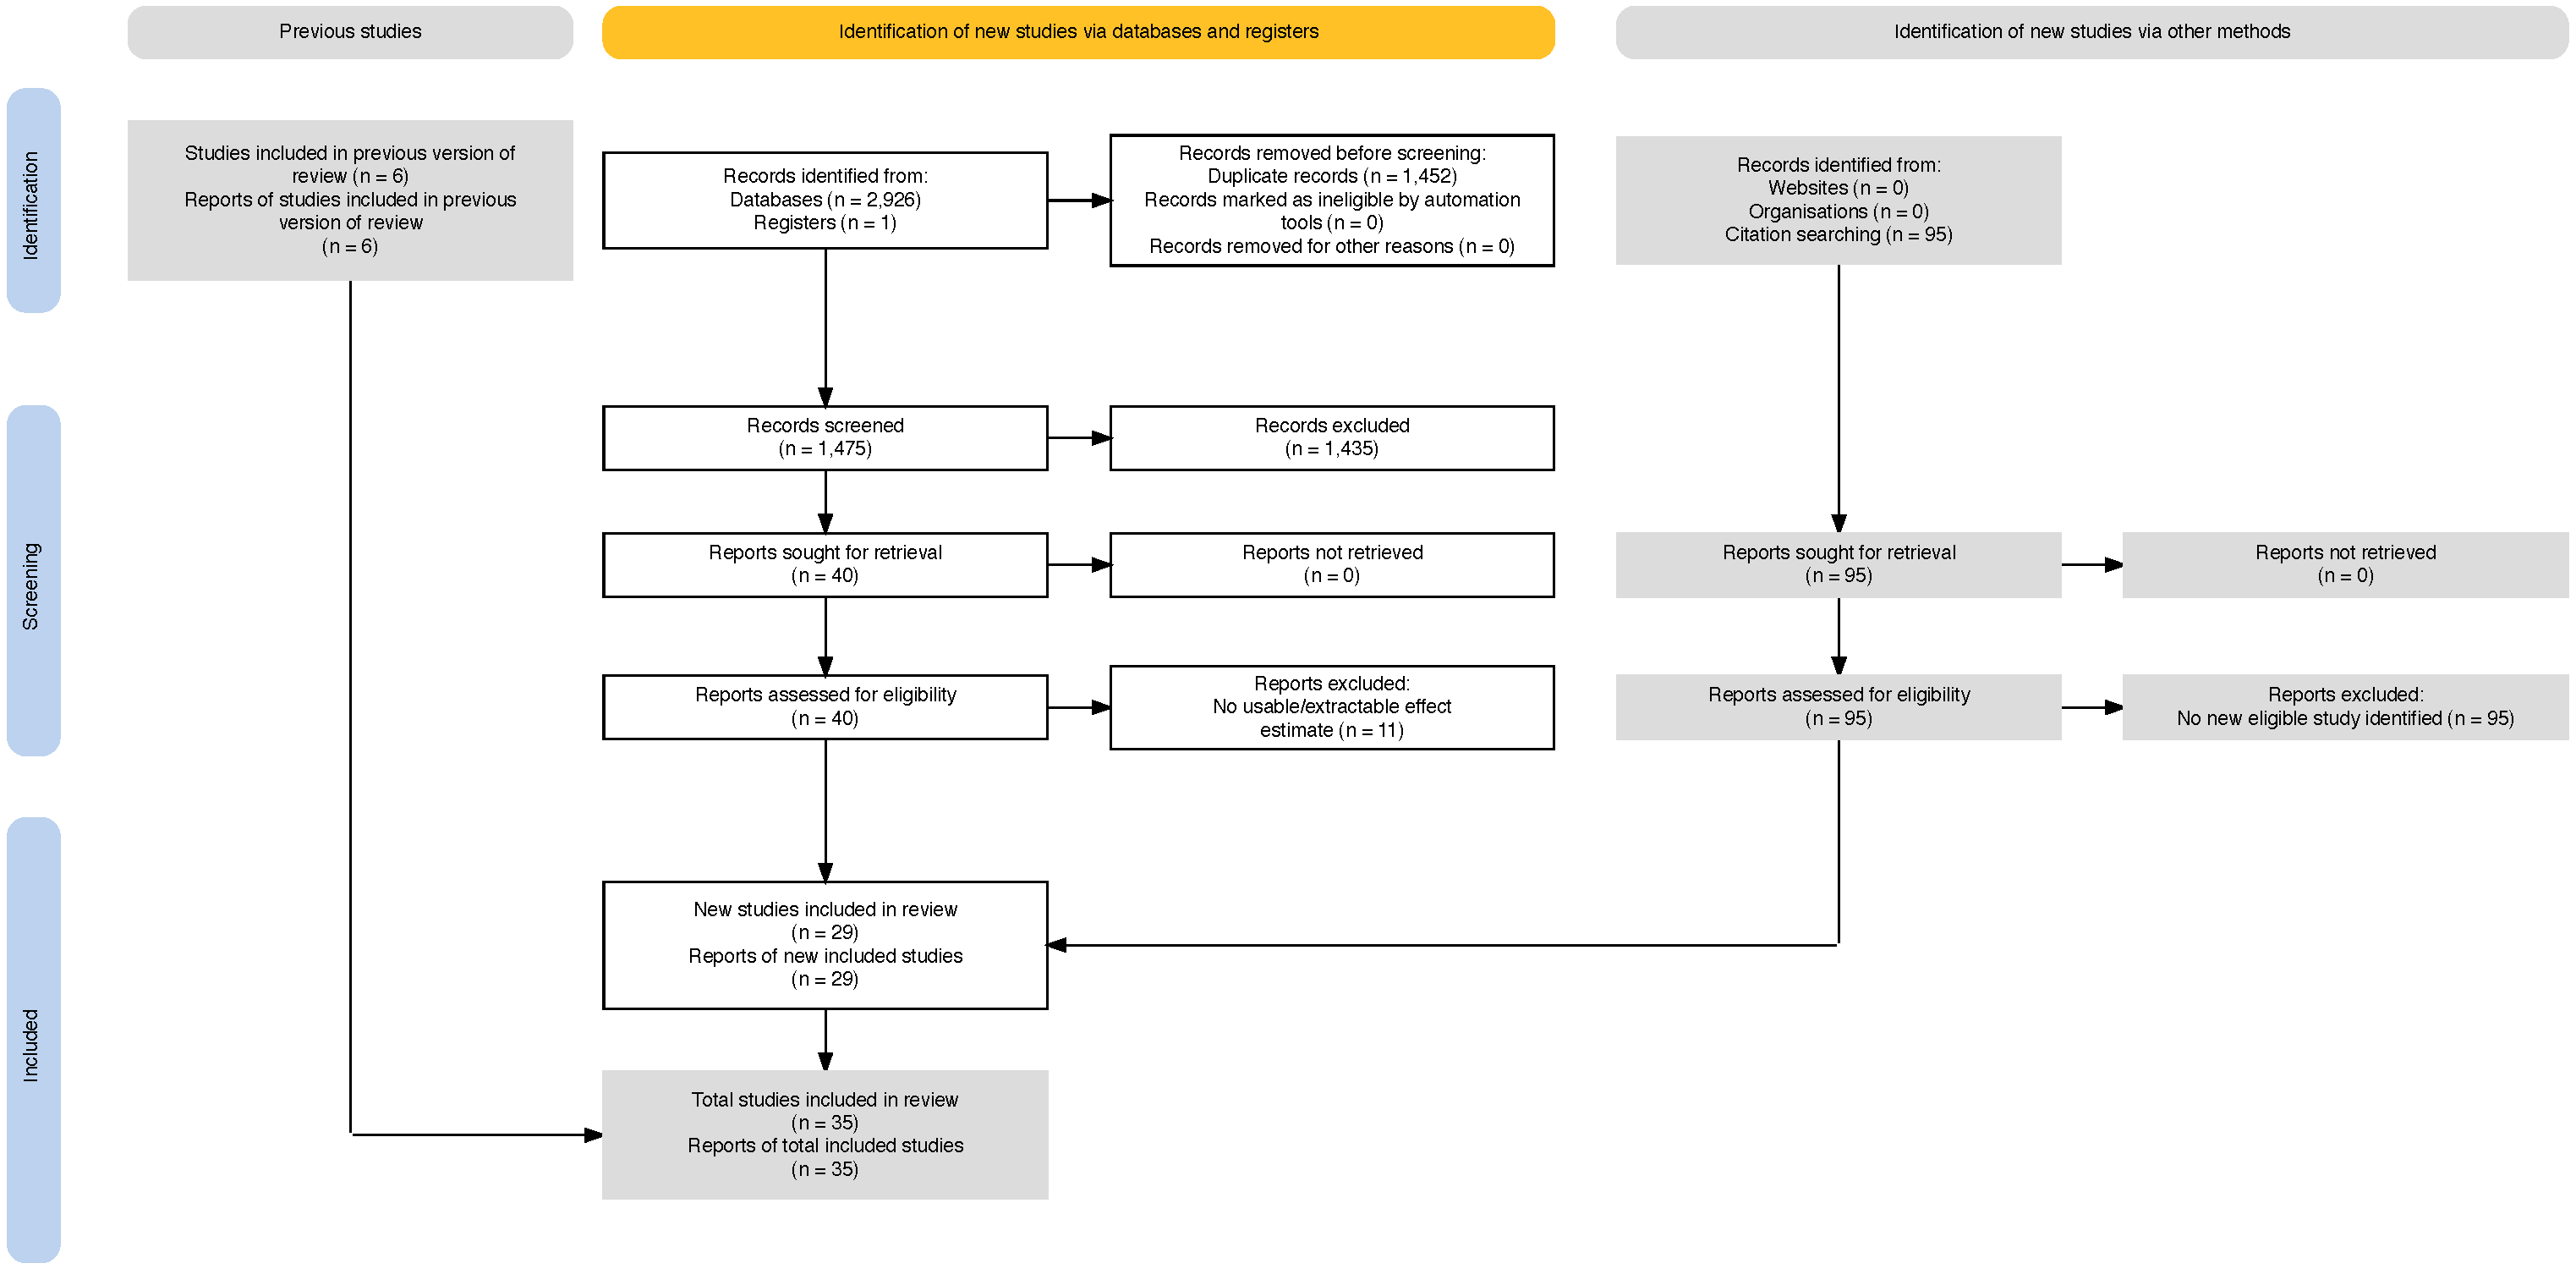
\includegraphics[width=1\linewidth,height=\textheight,keepaspectratio]{report_figs/prisma2020_flow.pdf}
\end{center}

\textbf{PRISMA 2020 flow.} Canonical PRISMA 2020 diagram (generated with
the \texttt{PRISMA2020} R package). Identification and de-duplication
counts are validated (2,926 database + 1 register records + 95 from
citation searching of Tariq 2018; 1,452 duplicates removed).
Screening-stage counts are \emph{provisional}, reconstructed from the
Elicit AI second-screen pending human dual screening per the protocol
(\texttt{PRISMA\_flow\_data.xlsx}): databases/registers arm 1,475
screened → 40 assessed → 11 full-text exclusions; the 95 other-methods
(citation) reports yielded no additional eligible study. Of the 35
included studies (29 new + 6 carried forward from Tariq 2018), 20
contribute a curated effect size to the Bayesian meta-analysis:
\textbf{11 in the primary comparison} (tetracyclines vs other
antibiotics) and \textbf{9 in the secondary comparison} (tetracyclines
vs no antibiotic).

\textbf{Flusso PRISMA 2020.} Diagramma PRISMA 2020 canonico (generato
con il pacchetto R \texttt{PRISMA2020}). I conteggi di identificazione e
deduplicazione sono validati (2.926 record da database + 1 registro + 95
da citation searching di Tariq 2018; 1.452 duplicati rimossi). I
conteggi della fase di screening sono \emph{provvisori}, ricostruiti dal
secondo screening AI di Elicit in attesa del doppio screening manuale
secondo il protocollo (\texttt{PRISMA\_flow\_data.xlsx}): braccio
database/registri 1.475 sottoposti a screening → 40 valutati → 11
esclusioni full-text; i 95 report da altri metodi (citation searching)
non hanno prodotto ulteriori studi eleggibili. Dei 35 studi inclusi (29
nuovi + 6 trasferiti da Tariq 2018), 20 contribuiscono con una stima
curata alla meta-analisi bayesiana: \textbf{11 nel confronto primario}
(tetracicline vs altri antibiotici) e \textbf{9 nel confronto
secondario} (tetracicline vs nessun antibiotico).

\subsection{\texorpdfstring{{Inter-rater agreement
(screening)}{Concordanza tra revisori
(screening)}}{Inter-rater agreement (screening)Concordanza tra revisori (screening)}}\label{inter-rater-agreement-screeningconcordanza-tra-revisori-screening}

The protocol (§16) requires two reviewers to screen titles/abstracts
independently, with agreement reported as Cohen's κ. Human dual
screening is \textbf{not yet complete}, so a \textbf{synthetic,
illustrative} decision log (\texttt{screening\_decisions.csv}, every row
tagged \texttt{SYNTHETIC\_ILLUSTRATIVE}) is included here purely to
demonstrate the calculation. The κ below is therefore illustrative only
and must be replaced by the real two-reviewer log (identical schema:
columns \texttt{reviewer1}/\texttt{reviewer2} holding include/exclude
per record); the chunk then reports the true agreement automatically.

Il protocollo (§16) richiede che due revisori effettuino lo screening di
titoli/abstract in modo indipendente, riportando la concordanza come κ
di Cohen. Il doppio screening manuale \textbf{non è ancora completo},
quindi qui è incluso un registro decisionale \textbf{sintetico e
illustrativo} (\texttt{screening\_decisions.csv}, con ogni riga
contrassegnata da \texttt{SYNTHETIC\_ILLUSTRATIVE}) al solo scopo di
dimostrare il calcolo. Il κ sottostante è quindi solo illustrativo e
deve essere sostituito dal registro reale dei due revisori (schema
identico: colonne \texttt{reviewer1}/\texttt{reviewer2} con
include/exclude per record); il blocco riporterà allora la concordanza
reale automaticamente.

\textbf{Cohen's κ = 0.54} (observed agreement 95.0\%; n = 1570 records)
--- \textbf{illustrative synthetic data; replace with the real
two-reviewer log}.

\subsection{\texorpdfstring{{Table 1. Characteristics of included
studies}{Tabella 1. Caratteristiche degli studi
inclusi}}{Table 1. Characteristics of included studiesTabella 1. Caratteristiche degli studi inclusi}}\label{table-1.-characteristics-of-included-studiestabella-1.-caratteristiche-degli-studi-inclusi}

{\def\LTcaptype{none} % do not increment counter
\begin{longtable}[]{@{}
  >{\raggedright\arraybackslash}p{(\linewidth - 14\tabcolsep) * \real{0.1488}}
  >{\raggedright\arraybackslash}p{(\linewidth - 14\tabcolsep) * \real{0.1736}}
  >{\raggedright\arraybackslash}p{(\linewidth - 14\tabcolsep) * \real{0.0661}}
  >{\raggedleft\arraybackslash}p{(\linewidth - 14\tabcolsep) * \real{0.0909}}
  >{\raggedright\arraybackslash}p{(\linewidth - 14\tabcolsep) * \real{0.1570}}
  >{\raggedright\arraybackslash}p{(\linewidth - 14\tabcolsep) * \real{0.1653}}
  >{\centering\arraybackslash}p{(\linewidth - 14\tabcolsep) * \real{0.0496}}
  >{\raggedleft\arraybackslash}p{(\linewidth - 14\tabcolsep) * \real{0.1488}}@{}}
\toprule\noalign{}
\begin{minipage}[b]{\linewidth}\raggedright
Study
\end{minipage} & \begin{minipage}[b]{\linewidth}\raggedright
Design
\end{minipage} & \begin{minipage}[b]{\linewidth}\raggedright
Setting
\end{minipage} & \begin{minipage}[b]{\linewidth}\raggedleft
N
\end{minipage} & \begin{minipage}[b]{\linewidth}\raggedright
Agent
\end{minipage} & \begin{minipage}[b]{\linewidth}\raggedright
Comparator
\end{minipage} & \begin{minipage}[b]{\linewidth}\centering
Adj.
\end{minipage} & \begin{minipage}[b]{\linewidth}\raggedleft
OR (95\% CI)
\end{minipage} \\
\midrule\noalign{}
\endhead
\bottomrule\noalign{}
\endlastfoot
(\citeproc{ref-Watson2018}{Watson et al. 2018}) & retrospective cohort &
HA & 1,237,537 & tetracycline class & reference category & Yes & 0.39
(0.31-0.51) \\
(\citeproc{ref-Baxter2008}{Baxter et al. 2008}) & matched case control &
HA & 4,493 & doxycycline & reference category & Yes & 0.41
(0.27-0.63) \\
(\citeproc{ref-Strom2017}{Ström et al. 2017}) & matched case control &
mixed & 584 & tetracycline & no antibiotic & No & 0.60 (0.14-2.55) \\
(\citeproc{ref-Webb2020}{Webb et al. 2020}) & retrospective cohort & HA
& 506,068 & doxycycline & reference category & Yes & 0.60 (0.33-1.10) \\
(\citeproc{ref-Doernberg2012}{Doernberg et al. 2012}) & retrospective
cohort & mixed & 2,734 & doxycycline & specific comparator & Yes & 0.73
(0.56-0.96) \\
(\citeproc{ref-Tilton2019}{Tilton and Johnson 2019}) & matched case
control & HA & 200 & doxycycline & no antibiotic & No & 0.76
(0.27-2.13) \\
(\citeproc{ref-OLeary2023}{O'Leary et al. 2023}) & retrospective cohort
& HA & 156,107 & doxycycline & specific comparator & Yes & 0.83
(0.70-0.99) \\
(\citeproc{ref-Tartof2015}{Tartof et al. 2015}) & retrospective cohort &
HA & 401,234 & tetracycline class & no antibiotic & No & 0.84
(0.63-1.10) \\
(\citeproc{ref-Delaney2007}{Delaney et al. 2007}) & matched case control
& CA & 13,563 & tetracycline class & no antibiotic & Yes & 0.90
(0.52-1.56) \\
(\citeproc{ref-Boven2026}{Boven et al. 2026}) & matched case control &
mixed & 398,080 & tetracycline class & reference category & Yes & 0.93
(0.80-1.09) \\
(\citeproc{ref-Carmichael2023}{Carmichael et al. 2023}) & retrospective
cohort & mixed & 50,861,011 & doxycycline & reference category & Yes &
0.94 (0.89-0.99) \\
(\citeproc{ref-Kuntz2011}{Kuntz et al. 2011}) & nested case control & CA
& 3,344 & tetracycline class & reference category & Yes & 0.94
(0.43-2.05) \\
(\citeproc{ref-Miller2023}{Miller et al. 2023}) & matched case control &
CA & 956,424 & doxycycline & reference category & Yes & 0.96
(0.90-1.03) \\
(\citeproc{ref-Guh2015}{Guh et al. 2017}) & matched case control & CA &
452 & tetracycline & no antibiotic & No & 1.00 (0.23-4.35) \\
(\citeproc{ref-Dial2008}{Dial et al. 2008}) & matched case control & CA
& NR & tetracycline class & no antibiotic & Yes & 1.10 (0.12-10.20) \\
(\citeproc{ref-Adams2017}{Adams et al. 2017}) & matched case control &
CA & 5,324 & tetracycline class & reference category & Yes & 1.26
(0.46-3.45) \\
(\citeproc{ref-Brown2016}{Brown et al. 2016}) & nested case control & HA
& 169,453 & tetracycline & no antibiotic & Yes & 1.26 (0.86-1.85) \\
(\citeproc{ref-Predrag2016}{Stojanović 2016}) & matched case control &
HA & 111 & tetracycline class & no antibiotic & No & 1.35 (0.22-8.47) \\
(\citeproc{ref-Yu2021}{Yu et al. 2021}) & matched case control & HA &
1,443 & tetracycline & no antibiotic & No & 2.90 (1.33-6.33) \\
(\citeproc{ref-Saito2025}{Saito et al. 2025}) & nested case control &
mixed & 24,585 & tetracycline class & reference category & Yes & 2.97
(2.44-3.62) \\
\end{longtable}
}

\textbf{Table 1.} Characteristics of the 20 studies contributing to the
Bayesian synthesis (11 vs other antibiotics; 9 vs no antibiotic; ordered
by odds ratio). N = analytic sample size (NR = not reported); Adj. =
adjusted estimate. The OR is the single curated effect size carried into
the meta-analysis; each study is identified by its bibliographic
citation.

\textbf{Tabella 1.} Caratteristiche dei 20 studi nella sintesi bayesiana
(11 vs altri antibiotici; 9 vs nessun antibiotico; ordinati per odds
ratio). N = dimensione campionaria analitica (NR = non riportata); Adj.
= stima aggiustata. L'OR è la singola stima d'effetto curata usata nella
meta-analisi; ogni studio è identificato dalla relativa citazione
bibliografica.

\subsection{\texorpdfstring{{Risk of bias (Newcastle-Ottawa
Scale)}{Rischio di bias (scala
Newcastle-Ottawa)}}{Risk of bias (Newcastle-Ottawa Scale)Rischio di bias (scala Newcastle-Ottawa)}}\label{risk-of-bias-newcastle-ottawa-scalerischio-di-bias-scala-newcastle-ottawa}

All 20 studies contributing to the synthesis are observational, so risk
of bias was assessed with the Newcastle-Ottawa Scale (NOS)
(\citeproc{ref-WellsNOS}{Wells et al. 2011}), using the
design-appropriate version (cohort or case-control; maximum 9 stars
across the Selection, Comparability and Outcome/Exposure domains).
Uniform decision rules were applied: the case-definition item was
credited only for laboratory-confirmed or independently validated
definitions (unvalidated ICD/claims algorithms were not); comparability
stars required matching or adjustment for age/sex (first star) and for
additional key confounders (second star), so studies whose curated
estimate is unadjusted beyond matching received one comparability star;
for cohorts, completeness of follow-up was credited only for closed
healthcare systems (HMO, claims or population registers). Overall
ratings: 7-9 stars = \textbf{low} risk of bias, 5-6 = \textbf{some
concerns}, 4 or fewer = \textbf{high}. Per-item scores and study-level
justifications are recorded in \texttt{nos\_assessment.csv}; the
study-level judgements are summarised as a traffic-light plot in Figure
9.

Tutti i 20 studi che contribuiscono alla sintesi sono osservazionali; il
rischio di bias è stato valutato con la scala Newcastle-Ottawa (NOS)
(\citeproc{ref-WellsNOS}{Wells et al. 2011}), nella versione appropriata
al disegno (coorte o caso-controllo; massimo 9 stelle nei domini
Selezione, Comparabilità ed Esito/Esposizione). Sono state applicate
regole decisionali uniformi: la definizione di caso è stata accreditata
solo se confermata in laboratorio o basata su codici validati (gli
algoritmi ICD/claims non validati non ricevono la stella); le stelle di
comparabilità richiedono appaiamento o aggiustamento per età/sesso
(prima stella) e per ulteriori confondenti chiave (seconda stella), per
cui gli studi la cui stima curata non è aggiustata oltre l'appaiamento
ricevono una sola stella; per le coorti, la completezza del follow-up è
stata accreditata solo per sistemi sanitari chiusi (HMO, claims o
registri di popolazione). Valutazioni complessive: 7-9 stelle = rischio
di bias \textbf{basso}, 5-6 = \textbf{alcune perplessità}, 4 o meno =
\textbf{alto}. I punteggi per singolo item e le giustificazioni per
studio sono registrati in \texttt{nos\_assessment.csv}; i giudizi per
studio sono riassunti come traffic-light plot nella Figura 9.

{\def\LTcaptype{none} % do not increment counter
\begin{longtable}[]{@{}
  >{\raggedright\arraybackslash}p{(\linewidth - 14\tabcolsep) * \real{0.1429}}
  >{\raggedright\arraybackslash}p{(\linewidth - 14\tabcolsep) * \real{0.1032}}
  >{\raggedright\arraybackslash}p{(\linewidth - 14\tabcolsep) * \real{0.0794}}
  >{\raggedleft\arraybackslash}p{(\linewidth - 14\tabcolsep) * \real{0.1270}}
  >{\raggedleft\arraybackslash}p{(\linewidth - 14\tabcolsep) * \real{0.1587}}
  >{\raggedleft\arraybackslash}p{(\linewidth - 14\tabcolsep) * \real{0.1825}}
  >{\raggedleft\arraybackslash}p{(\linewidth - 14\tabcolsep) * \real{0.0952}}
  >{\raggedright\arraybackslash}p{(\linewidth - 14\tabcolsep) * \real{0.1111}}@{}}
\toprule\noalign{}
\begin{minipage}[b]{\linewidth}\raggedright
Study
\end{minipage} & \begin{minipage}[b]{\linewidth}\raggedright
Design
\end{minipage} & \begin{minipage}[b]{\linewidth}\raggedright
Set
\end{minipage} & \begin{minipage}[b]{\linewidth}\raggedleft
Selection (0-4)
\end{minipage} & \begin{minipage}[b]{\linewidth}\raggedleft
Comparability (0-2)
\end{minipage} & \begin{minipage}[b]{\linewidth}\raggedleft
Outcome/Exposure (0-3)
\end{minipage} & \begin{minipage}[b]{\linewidth}\raggedleft
Total (0-9)
\end{minipage} & \begin{minipage}[b]{\linewidth}\raggedright
Overall RoB
\end{minipage} \\
\midrule\noalign{}
\endhead
\bottomrule\noalign{}
\endlastfoot
(\citeproc{ref-Adams2017}{Adams et al. 2017}) & case-control & primary &
4 & 2 & 3 & 9 & Low \\
(\citeproc{ref-Tartof2015}{Tartof et al. 2015}) & cohort & secondary & 4
& 2 & 3 & 9 & Low \\
(\citeproc{ref-Baxter2008}{Baxter et al. 2008}) & case-control & primary
& 3 & 2 & 3 & 8 & Low \\
(\citeproc{ref-Boven2026}{Boven et al. 2026}) & case-control & primary &
3 & 2 & 3 & 8 & Low \\
(\citeproc{ref-Brown2016}{Brown et al. 2016}) & case-control & secondary
& 3 & 2 & 3 & 8 & Low \\
(\citeproc{ref-Carmichael2023}{Carmichael et al. 2023}) & cohort &
primary & 3 & 2 & 3 & 8 & Low \\
(\citeproc{ref-Delaney2007}{Delaney et al. 2007}) & case-control &
secondary & 3 & 2 & 3 & 8 & Low \\
(\citeproc{ref-Dial2008}{Dial et al. 2008}) & case-control & secondary &
3 & 2 & 3 & 8 & Low \\
(\citeproc{ref-Guh2015}{Guh et al. 2017}) & case-control & secondary & 4
& 1 & 3 & 8 & Low \\
(\citeproc{ref-Kuntz2011}{Kuntz et al. 2011}) & case-control & primary &
3 & 2 & 3 & 8 & Low \\
(\citeproc{ref-Miller2023}{Miller et al. 2023}) & case-control & primary
& 3 & 2 & 3 & 8 & Low \\
(\citeproc{ref-OLeary2023}{O'Leary et al. 2023}) & cohort & primary & 4
& 2 & 2 & 8 & Low \\
(\citeproc{ref-Saito2025}{Saito et al. 2025}) & case-control & primary &
3 & 2 & 3 & 8 & Low \\
(\citeproc{ref-Strom2017}{Ström et al. 2017}) & case-control & secondary
& 4 & 1 & 3 & 8 & Low \\
(\citeproc{ref-Watson2018}{Watson et al. 2018}) & cohort & primary & 4 &
2 & 2 & 8 & Low \\
(\citeproc{ref-Webb2020}{Webb et al. 2020}) & cohort & primary & 4 & 2 &
2 & 8 & Low \\
(\citeproc{ref-Doernberg2012}{Doernberg et al. 2012}) & cohort & primary
& 3 & 2 & 2 & 7 & Low \\
(\citeproc{ref-Tilton2019}{Tilton and Johnson 2019}) & case-control &
secondary & 3 & 1 & 3 & 7 & Low \\
(\citeproc{ref-Yu2021}{Yu et al. 2021}) & case-control & secondary & 3 &
1 & 3 & 7 & Low \\
(\citeproc{ref-Predrag2016}{Stojanović 2016}) & case-control & secondary
& 2 & 1 & 3 & 6 & Some concerns \\
\end{longtable}
}

\textbf{Table 2.} Newcastle-Ottawa assessment of the 20 studies in the
synthesis (domain subtotals; maxima 4/2/3 stars, 9 overall). Selection
covers case/cohort definition, representativeness, comparison-group
selection and absence of the outcome at baseline (definition of controls
for case-control studies); Outcome/Exposure covers ascertainment of
outcome (cohorts) or exposure (case-control studies), comparability of
ascertainment across groups, and follow-up/non-response.

\textbf{Tabella 2.} Valutazione Newcastle-Ottawa dei 20 studi della
sintesi (subtotali per dominio; massimi 4/2/3 stelle, 9 complessive). La
selezione copre definizione di caso/coorte, rappresentatività, selezione
del gruppo di confronto e assenza dell'esito al baseline (definizione
dei controlli per i caso-controllo); Esito/Esposizione copre
l'accertamento dell'esito (coorti) o dell'esposizione (caso-controllo),
la comparabilità dell'accertamento tra i gruppi e il
follow-up/non-risposta.

\pandocbounded{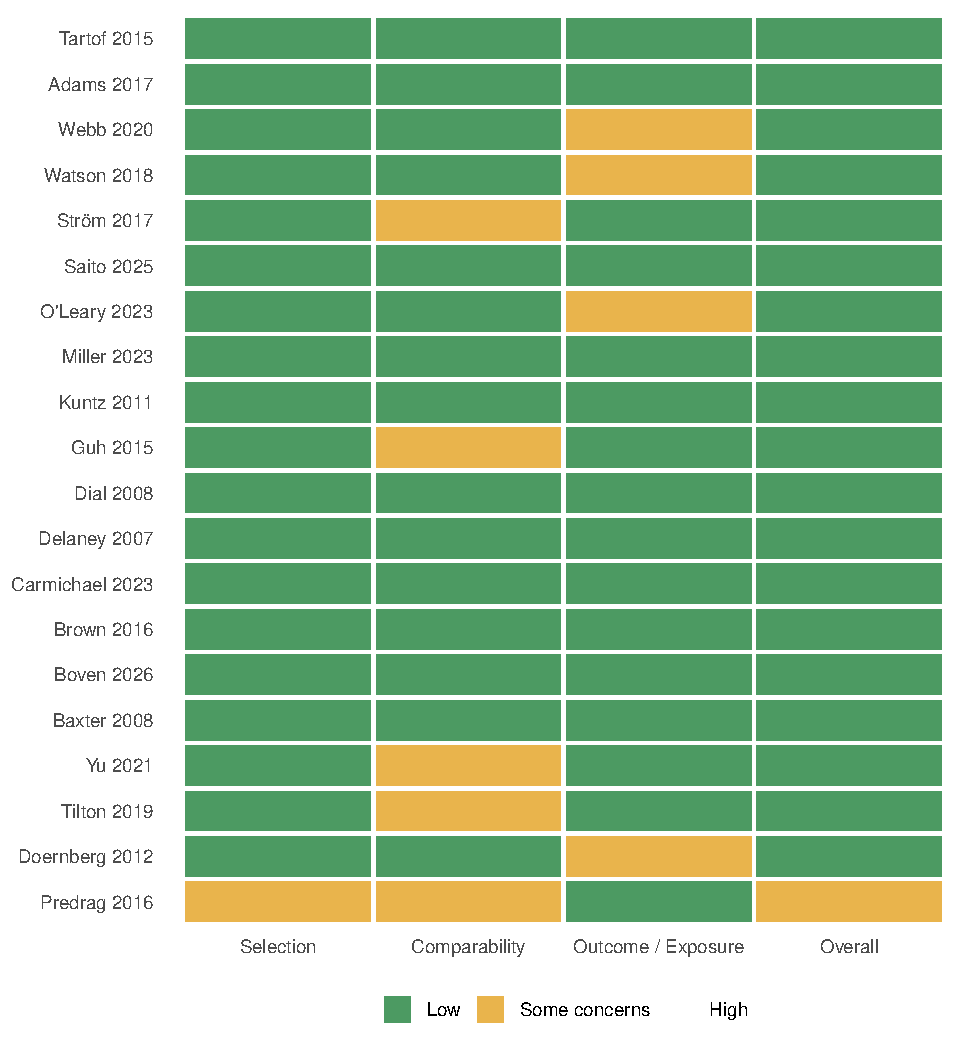
\includegraphics[keepaspectratio]{report_files/figure-pdf/rob-plot-1.pdf}}

\textbf{Traffic-light plot.} Domain-level risk-of-bias ratings. Domain
rules: Selection low if at least 3 of 4 stars; Comparability low with 2
stars, some concerns with 1; Outcome/Exposure low with 3 stars, some
concerns with 2. Overall: 7-9 low, 5-6 some concerns, 4 or fewer high.

\textbf{Traffic-light plot.} Valutazioni di rischio di bias per dominio.
Regole: Selezione bassa con almeno 3 stelle su 4; Comparabilità bassa
con 2 stelle, alcune perplessità con 1; Esito/Esposizione bassa con 3
stelle, alcune perplessità con 2. Complessivo: 7-9 basso, 5-6 alcune
perplessità, 4 o meno alto.

19 of 20 studies reach 7 or more stars (low risk of bias). Recurring
limitations are case definitions based on unvalidated diagnostic codes
(selection), hospital-based controls in smaller case-control studies
(selection), reliance on unadjusted per-drug estimates (comparability),
and uncertain completeness of post-discharge outcome capture in
hospital-discharge cohorts (outcome). For the six studies carried
forward from Tariq et al.~(2018), our independent scores (median 8,
range 7-9) are consistent with theirs (median 7, range 7-8)
(\citeproc{ref-Tariq2018}{Tariq and Khanna 2018}).

The pre-specified sensitivity analysis excluding studies at higher risk
of bias (NOS below 7) removes only Predrag 2016: the primary estimate is
unchanged because all 11 antibiotic-comparator studies are low risk (OR
0.86 (0.60--1.23)), and the secondary, no-antibiotic comparison becomes
OR 1.05 (0.74--1.54) (k = 8). Conclusions are therefore robust to study
quality as assessed here.

19 studi su 20 raggiungono almeno 7 stelle (basso rischio di bias). Le
limitazioni ricorrenti sono definizioni di caso basate su codici
diagnostici non validati (selezione), controlli ospedalieri negli studi
caso-controllo più piccoli (selezione), affidamento a stime per singolo
farmaco non aggiustate (comparabilità) e incerta completezza della
cattura dell'esito dopo la dimissione nelle coorti ospedaliere (esito).
Per i sei studi trasferiti da Tariq et al.~(2018), i nostri punteggi
indipendenti (mediana 8, intervallo 7-9) sono coerenti con i loro
(mediana 7, intervallo 7-8) (\citeproc{ref-Tariq2018}{Tariq and Khanna
2018}).

L'analisi di sensibilità pre-specificata che esclude gli studi a maggior
rischio di bias (NOS inferiore a 7) rimuove solo Predrag 2016: la stima
primaria è invariata perché tutti gli 11 studi con comparatore
antibiotico sono a basso rischio (OR 0.86 (0.60--1.23)), e il confronto
secondario (vs nessun antibiotico) diventa OR 1.05 (0.74--1.54) (k = 8).
Le conclusioni sono quindi robuste rispetto alla qualità degli studi
così come valutata qui.

\begin{tcolorbox}[enhanced jigsaw, arc=.35mm, bottomrule=.15mm, bottomtitle=1mm, breakable, colback=white, colbacktitle=quarto-callout-note-color!10!white, colframe=quarto-callout-note-color-frame, coltitle=black, left=2mm, leftrule=.75mm, opacityback=0, opacitybacktitle=0.6, rightrule=.15mm, title=\textcolor{quarto-callout-note-color}{\faInfo}\hspace{0.5em}{Note}, titlerule=0mm, toprule=.15mm, toptitle=1mm]

\textbf{Protocol deviation --- no randomised trials included.} The
protocol pre-specified RCTs as an eligible design, with a study-design
stratification (observational vs RCT) and a Cochrane \textbf{RoB 2}
appraisal for any trials. No RCT met the inclusion criteria: all 20
studies in the synthesis are observational. The observational-vs-RCT
stratum and the RoB 2 appraisal are therefore not applicable and were
not performed, and the design meta-regression is restricted to
observational designs (case-control vs cohort).

\textbf{Deviazione dal protocollo --- nessuno studio randomizzato
incluso.} Il protocollo prevedeva gli RCT tra i disegni eleggibili, con
una stratificazione per disegno (osservazionale vs RCT) e la valutazione
Cochrane \textbf{RoB 2} per eventuali trial. Nessun RCT ha soddisfatto i
criteri di inclusione: tutti i 20 studi della sintesi sono
osservazionali. Lo strato osservazionale-vs-RCT e la valutazione RoB 2
non sono quindi applicabili e non sono stati eseguiti, e la
meta-regressione per disegno è limitata ai disegni osservazionali
(caso-controllo vs coorte).

\end{tcolorbox}

\subsection{\texorpdfstring{{Methods}{Metodi}}{MethodsMetodi}}\label{methodsmetodi}

Hierarchical random-effects model on the log-odds scale:
\[y_i \sim \text{Normal}(\theta_i, s_i^2), \qquad \theta_i \sim \text{Normal}(\mu, \tau^2).\]
Primary prior \(\mu \sim \text{Normal}(0, 1^2)\); heterogeneity prior
\(\tau \sim \text{Half-Normal}(0, 0.5)\). Posteriors were computed
exactly by numerical integration (\texttt{bayesmeta}) and independently
confirmed by Hamiltonian Monte Carlo (\texttt{brms}/Stan, 4 chains). We
report the pooled odds ratio (OR = exp \(\mu\)) with a 95\% credible
interval (CrI), the between-study SD \(\tau\), the predictive interval
for a new study, and the posterior probabilities P(OR\textless1) and
P(OR\textless0.80). A pre-specified prior-sensitivity analysis used
vague, sceptical and literature-informed priors.

Modello gerarchico a effetti casuali su scala log-odds:
\[y_i \sim \text{Normale}(\theta_i, s_i^2), \qquad \theta_i \sim \text{Normale}(\mu, \tau^2).\]
Prior primario \(\mu \sim \text{Normale}(0, 1^2)\); prior
sull'eterogeneità \(\tau \sim \text{Half-Normale}(0, 0.5)\). Le
distribuzioni a posteriori sono state calcolate in modo esatto per
integrazione numerica (\texttt{bayesmeta}) e confermate in modo
indipendente con Hamiltonian Monte Carlo (\texttt{brms}/Stan, 4 catene).
Riportiamo l'odds ratio aggregato (OR = exp \(\mu\)) con intervallo di
credibilità (ICr) al 95\%, la deviazione standard tra studi \(\tau\),
l'intervallo predittivo per un nuovo studio e le probabilità a
posteriori P(OR\textless1) e P(OR\textless0,80). Un'analisi di
sensibilità sui prior pre-specificata ha usato prior vago, scettico e
informato dalla letteratura.

\subsection{\texorpdfstring{{Primary result (11 studies)}{Risultato
primario (11
studi)}}{Primary result (11 studies)Risultato primario (11 studi)}}\label{primary-result-11-studiesrisultato-primario-11-studi}

Pooled odds ratio (tetracyclines vs other antibiotics) {0.86
(0.60--1.23)}

The 95\% credible interval crosses 1. The posterior probability of any
protective effect is \textbf{P(OR\textless1) = 0.81}, and the
probability of a clinically meaningful effect is
\textbf{P(OR\textless0.80) = 0.35}. Between-study heterogeneity is
substantial (\(\tau\) = 0.55 (0.34--0.83); I² = 98\% (95\% CrI
96--99\%)): the predictive interval for a future study spans OR
0.25--2.88.

Odds ratio aggregato (tetracicline vs altri antibiotici) {0.86
(0.60--1.23)}

L'intervallo di credibilità al 95\% attraversa 1. La probabilità a
posteriori di un qualsiasi effetto protettivo è \textbf{P(OR\textless1)
= 0.81}, e la probabilità di un effetto clinicamente rilevante è
\textbf{P(OR\textless0,80) = 0.35}. L'eterogeneità tra studi è
sostanziale (\(\tau\) = 0.55 (0.34--0.83); I² = 98\% (95\% CrI
96--99\%)): l'intervallo predittivo per uno studio futuro va da OR
0.25--2.88.

\begin{figure}

\centering{

\pandocbounded{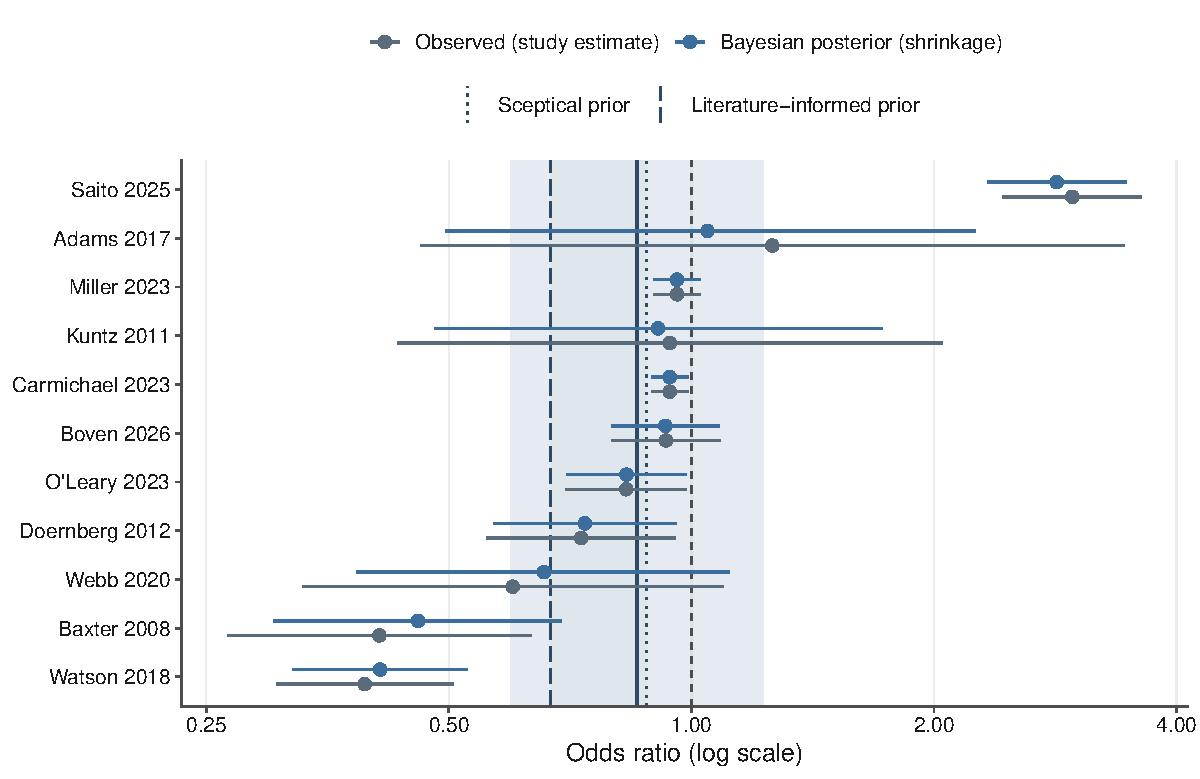
\includegraphics[keepaspectratio]{report_files/figure-pdf/fig-forest-1.pdf}}

}

\caption{\label{fig-forest}}

\end{figure}%

\textbf{Figure 1.} Study-level odds ratios (primary set, 11 studies with
antibiotic comparators). Gray = observed estimates; blue = Bayesian
posterior (shrinkage) estimates, pulled toward the pooled mean. The navy
line and blue band show the pooled OR (primary prior) and 95\% credible
interval. The dotted and long-dashed vertical lines mark the pooled OR
under the sceptical and literature-informed priors; the faint outer band
is the prior-sensitivity range.

\textbf{Figura 1.} Odds ratio per studio (set primario, 11 studi con
comparatori antibiotici). Grigio = stime osservate; blu = stime a
posteriori bayesiane (shrinkage), attratte verso la media aggregata. La
linea navy e la banda blu indicano l'OR aggregato (prior primario) e
l'ICr al 95\%. Le linee verticali punteggiata e tratteggiata indicano
l'OR aggregato con i prior scettico e informato dalla letteratura; la
banda esterna tenue è l'intervallo di sensibilità ai prior.

\subsection{\texorpdfstring{{Prior sensitivity}{Sensibilità ai
prior}}{Prior sensitivitySensibilità ai prior}}\label{prior-sensitivitysensibilituxe0-ai-prior}

The estimate is stable across data-dominated priors (primary, vague,
sceptical) but shifts toward protection under the literature-informed
prior centred on the earlier Tariq (2018) estimate of OR 0.62 ---
i.e.~that conclusion is driven by prior belief, not the new data.

La stima è stabile tra i prior dominati dai dati (primario, vago,
scettico) ma si sposta verso la protezione con il prior informato dalla
letteratura, centrato sulla stima precedente di Tariq (2018), OR 0,62
--- cioè quella conclusione è guidata dalla convinzione a priori, non
dai nuovi dati.

{

\begin{longtable}[]{@{}
  >{\raggedright\arraybackslash}p{(\linewidth - 6\tabcolsep) * \real{0.4507}}
  >{\centering\arraybackslash}p{(\linewidth - 6\tabcolsep) * \real{0.2535}}
  >{\centering\arraybackslash}p{(\linewidth - 6\tabcolsep) * \real{0.1268}}
  >{\centering\arraybackslash}p{(\linewidth - 6\tabcolsep) * \real{0.1690}}@{}}

\caption{\label{tbl-prior-en}}

\tabularnewline

\toprule\noalign{}
\begin{minipage}[b]{\linewidth}\raggedright
Prior on μ
\end{minipage} & \begin{minipage}[b]{\linewidth}\centering
OR (95\% CrI)
\end{minipage} & \begin{minipage}[b]{\linewidth}\centering
P(OR\textless1)
\end{minipage} & \begin{minipage}[b]{\linewidth}\centering
P(OR\textless0.80)
\end{minipage} \\
\midrule\noalign{}
\endhead
\bottomrule\noalign{}
\endlastfoot
Primary --- N(0, 1²) & 0.86 (0.60--1.23) & 0.81 & 0.35 \\
Vague --- N(0, 10²) & 0.85 (0.59--1.23) & 0.82 & 0.36 \\
Sceptical --- N(0, 0.35²) & 0.88 (0.64--1.21) & 0.79 & 0.27 \\
Literature --- N(log 0.62, 0.10²) & 0.67 (0.56--0.80) & 1.00 & 0.98 \\

\end{longtable}

}

{

\begin{longtable}[]{@{}
  >{\raggedright\arraybackslash}p{(\linewidth - 6\tabcolsep) * \real{0.4583}}
  >{\centering\arraybackslash}p{(\linewidth - 6\tabcolsep) * \real{0.2500}}
  >{\centering\arraybackslash}p{(\linewidth - 6\tabcolsep) * \real{0.1250}}
  >{\centering\arraybackslash}p{(\linewidth - 6\tabcolsep) * \real{0.1667}}@{}}

\caption{\label{tbl-prior-it}}

\tabularnewline

\toprule\noalign{}
\begin{minipage}[b]{\linewidth}\raggedright
Prior su μ
\end{minipage} & \begin{minipage}[b]{\linewidth}\centering
OR (ICr 95\%)
\end{minipage} & \begin{minipage}[b]{\linewidth}\centering
P(OR\textless1)
\end{minipage} & \begin{minipage}[b]{\linewidth}\centering
P(OR\textless0,80)
\end{minipage} \\
\midrule\noalign{}
\endhead
\bottomrule\noalign{}
\endlastfoot
Primario --- N(0, 1²) & 0.86 (0.60--1.23) & 0.81 & 0.35 \\
Vago --- N(0, 10²) & 0.85 (0.59--1.23) & 0.82 & 0.36 \\
Scettico --- N(0, 0,35²) & 0.88 (0.64--1.21) & 0.79 & 0.27 \\
Letteratura --- N(log 0,62, 0,10²) & 0.67 (0.56--0.80) & 1.00 & 0.98 \\

\end{longtable}

}

\subsection{\texorpdfstring{{Prior-data conflict}{Conflitto
prior-dati}}{Prior-data conflictConflitto prior-dati}}\label{prior-data-conflictconflitto-prior-dati}

Because the literature-informed prior is the only assumption under which
the result becomes confidently protective, we formally check whether it
conflicts with the updated data. Using the Box / Marshall-Spiegelhalter
measure, we compare the prior for μ --- N(log 0.62, 0.10²), i.e.~OR 0.62
--- against the data-only estimate (vague-prior posterior: OR 0.85,
log-scale mean -0.16, SD 0.19). The conflict statistic is z = -1.50
(two-sided p = 0.13), indicating \textbf{mild tension but no formal
conflict}. The literature prior is more optimistic than the updated
evidence, but the gap is within sampling variation. Its influence on the
pooled estimate comes mainly from being far narrower (SD 0.10) than the
data-only posterior (SD 0.19) rather than from statistical
incompatibility with the data.

Poiché il prior informato dalla letteratura è l'unica assunzione sotto
cui il risultato diventa decisamente protettivo, verifichiamo
formalmente se sia in conflitto con i dati aggiornati. Con la misura di
Box / Marshall-Spiegelhalter confrontiamo il prior per μ --- N(log 0,62,
0,10²), cioè OR 0,62 --- con la stima basata sui soli dati (posteriori
con prior vago: OR 0.85, media log -0.16, SD 0.19). La statistica di
conflitto è z = -1.50 (p bilaterale = 0.13), indicando \textbf{una lieve
tensione ma nessun conflitto formale}. Il prior della letteratura è più
ottimistico delle evidenze aggiornate, ma la differenza rientra nella
variabilità campionaria. La sua influenza deriva soprattutto dall'essere
molto più stretto (SD 0,10) della posteriori basata sui dati (SD 0.19),
non da un'incompatibilità statistica con i dati.

\subsection{\texorpdfstring{{MCMC confirmation \& convergence}{Conferma
MCMC e
convergenza}}{MCMC confirmation \& convergenceConferma MCMC e convergenza}}\label{mcmc-confirmation-convergenceconferma-mcmc-e-convergenza}

\textbf{Sampling.} The confirmatory fit uses Hamiltonian Monte Carlo
(Stan, via \texttt{brms}) with the same priors as the exact model: 4
chains of 4,000 iterations (1,000 warmup), giving 12,000 post-warmup
draws, with \texttt{adapt\_delta\ =\ 0.99} to handle the funnel-shaped
geometry typical of hierarchical models with few studies. The run
produced \textbf{0 divergent transitions} and 0 iterations at the
maximum tree depth, so the sampler explored the posterior without
numerical failures.

\textbf{Convergence.} R-hat compares within- and between-chain variance;
both parameters are essentially 1.00 (max 1.000, below the conventional
1.01 threshold), so the four chains have converged to the same target
distribution. Bulk ESS (2516 for μ, 3217 for τ) and tail ESS (3702 /
5375) are large, meaning both the centre of the posterior and the
extreme quantiles --- on which the 95\% credible interval and
P(OR\textless1) depend --- rest on the equivalent of thousands of
independent draws; the Monte Carlo standard error of the pooled log-OR
is only 0.004. The trace plots (Figure 2) confirm this visually: the
four chains overlap around stable levels, with no trends, drift or
sticking.

\textbf{Agreement between engines.} \texttt{bayesmeta} computes the
posterior by deterministic numerical integration (no Monte Carlo error
at all), whereas \texttt{brms}/Stan approximates it by sampling. That
the two agree closely (table below) shows the reported posterior is a
property of the model and the data rather than of the computational
method --- and it validates the exact \texttt{bayesmeta} posteriors used
throughout this report.

\textbf{Campionamento.} Il modello di conferma usa Hamiltonian Monte
Carlo (Stan, tramite \texttt{brms}) con gli stessi prior del modello
esatto: 4 catene da 4.000 iterazioni (1.000 di warmup), per un totale di
12.000 draw post-warmup, con \texttt{adapt\_delta\ =\ 0,99} per gestire
la geometria ``a imbuto'' tipica dei modelli gerarchici con pochi studi.
L'esecuzione ha prodotto \textbf{0 transizioni divergenti} e 0
iterazioni alla profondità massima dell'albero: il campionatore ha
esplorato la posteriori senza problemi numerici.

\textbf{Convergenza.} R-hat confronta la varianza entro e tra le catene;
entrambi i parametri sono sostanzialmente a 1,00 (max 1.000, sotto la
soglia convenzionale di 1,01), quindi le quattro catene sono convergenti
alla stessa distribuzione obiettivo. Gli ESS bulk (2516 per μ, 3217 per
τ) e tail (3702 / 5375) sono ampi: sia il centro della posteriori sia i
quantili estremi --- da cui dipendono l'ICr al 95\% e P(OR\textless1)
--- poggiano sull'equivalente di migliaia di draw indipendenti; l'errore
standard Monte Carlo del log-OR aggregato è solo 0.004. I trace plot
(Figura 2) lo confermano visivamente: le quattro catene si sovrappongono
attorno a livelli stabili, senza trend, deriva o blocchi.

\textbf{Accordo tra i motori.} \texttt{bayesmeta} calcola la posteriori
per integrazione numerica deterministica (senza alcun errore Monte
Carlo), mentre \texttt{brms}/Stan la approssima per campionamento. Il
fatto che i due concordino strettamente (tabella sotto) mostra che la
posteriori riportata è una proprietà del modello e dei dati, non del
metodo computazionale --- e convalida le posteriori esatte di
\texttt{bayesmeta} usate in tutto il report.

{

\begin{longtable}[]{@{}lcccc@{}}

\caption{\label{tbl-confirm-en}}

\tabularnewline

\toprule\noalign{}
Method & OR (95\% CrI) & τ & P(OR\textless1) & P(OR\textless0.80) \\
\midrule\noalign{}
\endhead
\bottomrule\noalign{}
\endlastfoot
bayesmeta (exact) & 0.86 (0.60--1.23) & 0.55 & 0.81 & 0.35 \\
brms (MCMC) & 0.85 (0.60--1.23) & 0.55 & 0.81 & 0.36 \\

\end{longtable}

}

{

\begin{longtable}[]{@{}lcccc@{}}

\caption{\label{tbl-confirm-en}}

\tabularnewline

\toprule\noalign{}
Parameter & R-hat & Bulk ESS & Tail ESS & MCSE (mean) \\
\midrule\noalign{}
\endhead
\bottomrule\noalign{}
\endlastfoot
μ (log-OR) & 1.000 & 2516 & 3702 & 0.004 \\
τ (heterogeneity SD) & 1.000 & 3217 & 5375 & 0.002 \\

\end{longtable}

}

{

\begin{longtable}[]{@{}lcccc@{}}

\caption{\label{tbl-confirm-it}}

\tabularnewline

\toprule\noalign{}
Metodo & OR (ICr 95\%) & τ & P(OR\textless1) & P(OR\textless0,80) \\
\midrule\noalign{}
\endhead
\bottomrule\noalign{}
\endlastfoot
bayesmeta (exact) & 0.86 (0.60--1.23) & 0.55 & 0.81 & 0.35 \\
brms (MCMC) & 0.85 (0.60--1.23) & 0.55 & 0.81 & 0.36 \\

\end{longtable}

}

{

\begin{longtable}[]{@{}lcccc@{}}

\caption{\label{tbl-confirm-it}}

\tabularnewline

\toprule\noalign{}
Parametro & R-hat & ESS bulk & ESS tail & MCSE (media) \\
\midrule\noalign{}
\endhead
\bottomrule\noalign{}
\endlastfoot
μ (log-OR) & 1.000 & 2516 & 3702 & 0.004 \\
τ (SD eterogeneità) & 1.000 & 3217 & 5375 & 0.002 \\

\end{longtable}

}

\begin{figure}

\centering{

\pandocbounded{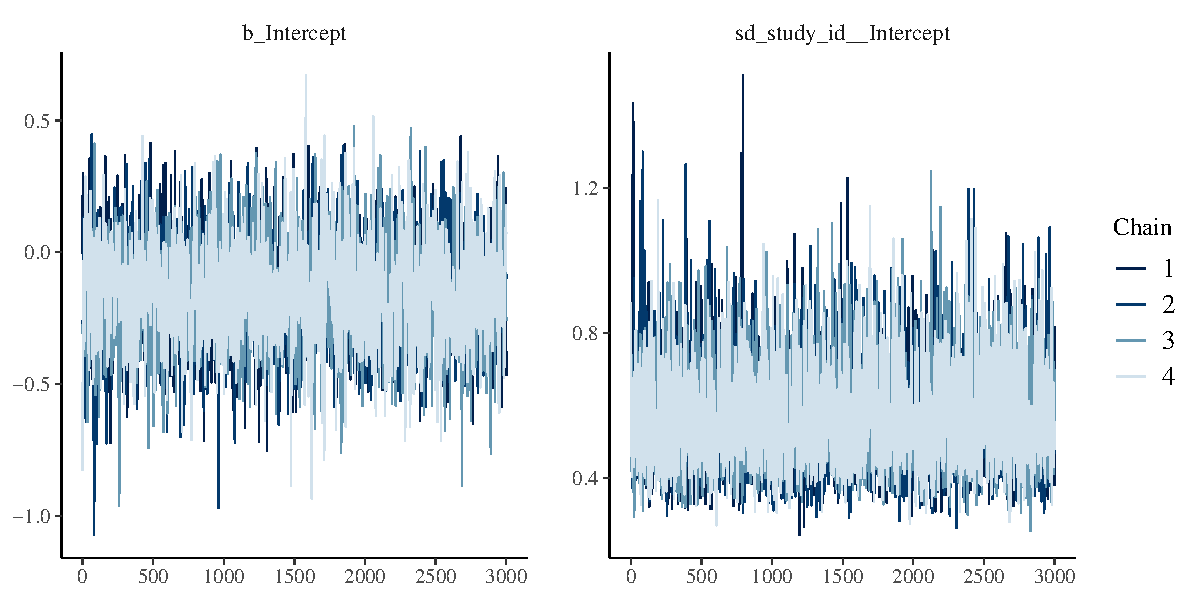
\includegraphics[keepaspectratio]{report_files/figure-pdf/fig-trace-1.pdf}}

}

\caption{\label{fig-trace}}

\end{figure}%

\textbf{Figure 2.} MCMC trace plots for the four chains (pooled log-OR μ
and heterogeneity SD τ). Overlapping chains fluctuating around stable
levels --- with no trends, drift or sticking --- indicate good mixing
and stationarity.

\textbf{Figura 2.} Trace plot MCMC per le quattro catene (log-OR
aggregato μ e SD dell'eterogeneità τ). Catene sovrapposte che oscillano
attorno a livelli stabili --- senza trend, deriva o blocchi --- indicano
buon mixing e stazionarietà.

\subsection{\texorpdfstring{{Small-study effects}{Effetti dei piccoli
studi}}{Small-study effectsEffetti dei piccoli studi}}\label{small-study-effectseffetti-dei-piccoli-studi}

With k = 11 studies (meeting the pre-specified ≥10 threshold), a
contour-enhanced funnel plot and Egger's regression test assess funnel
asymmetry. There is \textbf{no evidence of asymmetry} (Egger z = -0.28,
p = 0.78); the studies scatter fairly symmetrically about the pooled
effect. Given the observational evidence base and modest k, this is
reassuring but not decisive.

Con k = 11 studi (soglia pre-specificata ≥10), un funnel plot
contour-enhanced e il test di regressione di Egger valutano
l'asimmetria. \textbf{Non vi è evidenza di asimmetria} (Egger z = -0.28,
p = 0.78); gli studi si distribuiscono in modo abbastanza simmetrico
attorno all'effetto aggregato. Data la natura osservazionale e il k
contenuto, è rassicurante ma non decisivo.

\begin{figure}

\centering{

\pandocbounded{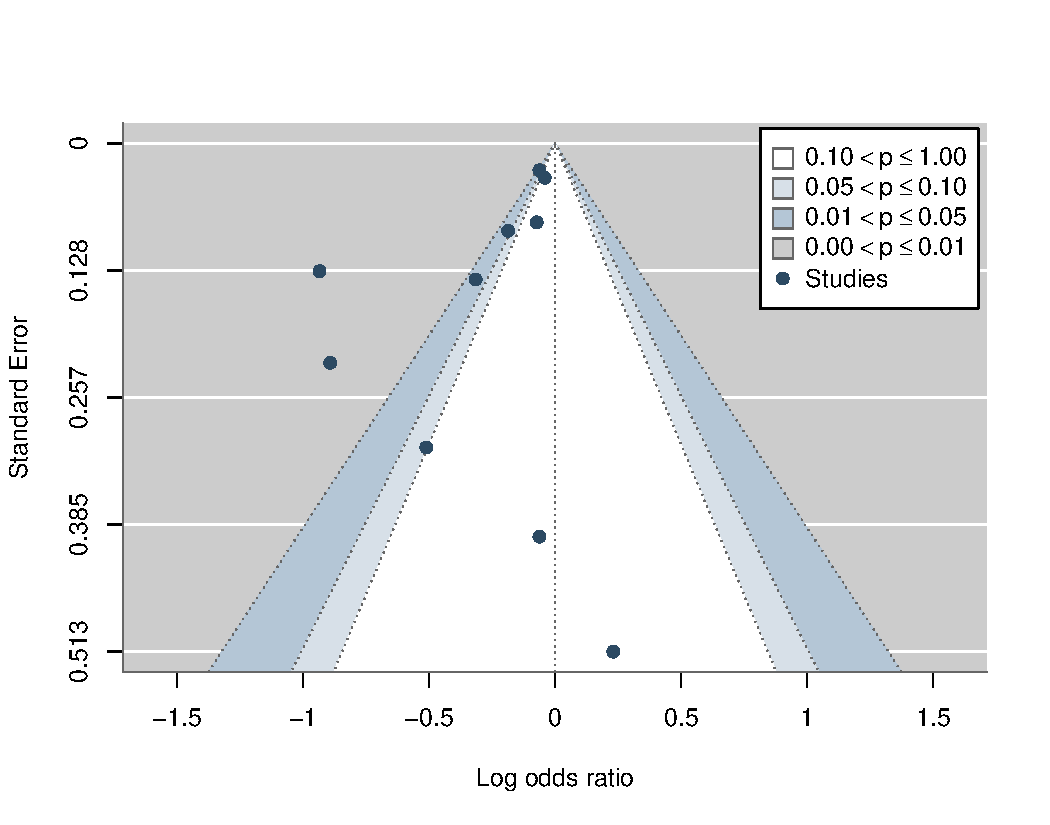
\includegraphics[keepaspectratio]{report_files/figure-pdf/fig-funnel-1.pdf}}

}

\caption{\label{fig-funnel}}

\end{figure}%

\textbf{Figure 3.} Contour-enhanced funnel plot; shaded bands mark the p
= 0.10 / 0.05 / 0.01 regions.

\textbf{Figura 3.} Funnel plot contour-enhanced; le bande indicano le
regioni p = 0,10 / 0,05 / 0,01.

\subsection{\texorpdfstring{{Leave-one-out}{Analisi
leave-one-out}}{Leave-one-outAnalisi leave-one-out}}\label{leave-one-outanalisi-leave-one-out}

No single study drives the pooled estimate: removing any one study
leaves the pooled OR between 0.75 and 0.93, always below 1. The most
influential study is Saito 2025 (a harmful outlier); dropping it moves
the OR most toward protection, while dropping the protective Watson 2018
moves it toward the null. The qualitative conclusion is stable
throughout.

Nessun singolo studio determina la stima aggregata: rimuovendo un
qualsiasi studio l'OR aggregato resta tra 0.75 e 0.93, sempre inferiore
a 1. Lo studio più influente è Saito 2025 (un outlier sfavorevole): la
sua rimozione sposta l'OR verso la protezione, mentre rimuovere il
protettivo Watson 2018 lo sposta verso l'assenza di effetto. La
conclusione qualitativa resta stabile.

\begin{figure}

\centering{

\pandocbounded{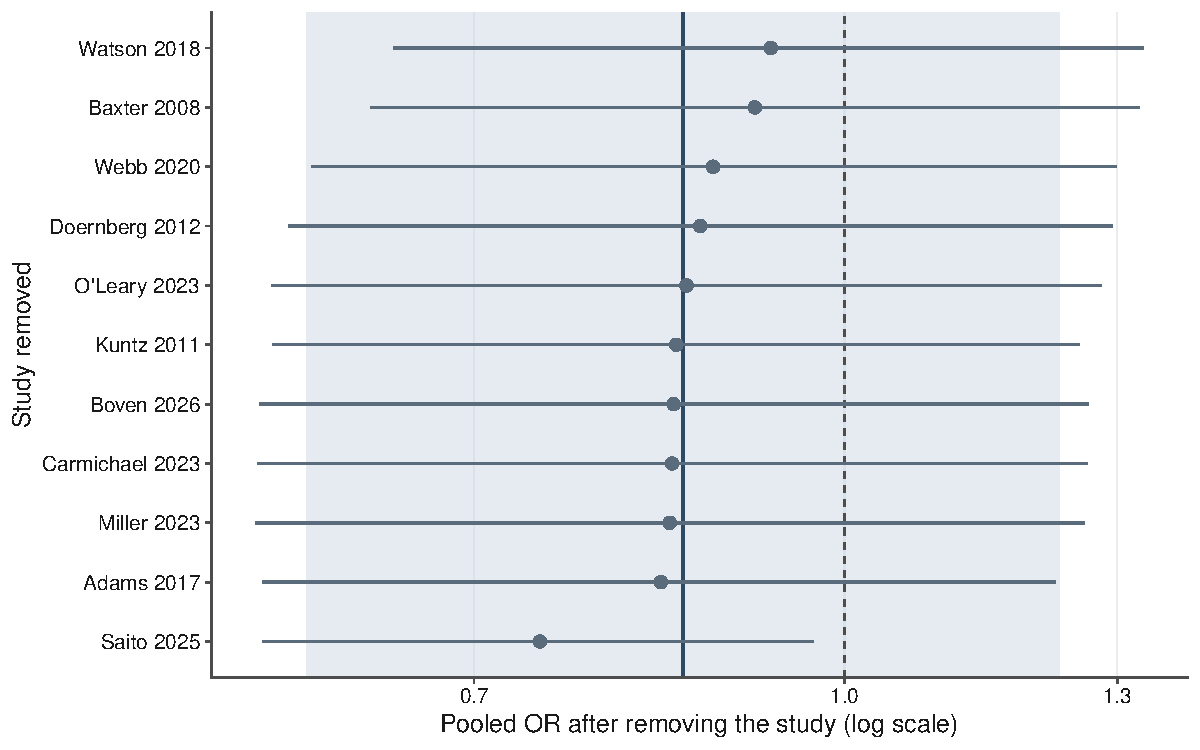
\includegraphics[keepaspectratio]{report_files/figure-pdf/fig-loo-1.pdf}}

}

\caption{\label{fig-loo}}

\end{figure}%

\textbf{Figure 4.} Leave-one-out pooled OR; the blue line and band are
the full k = 11 estimate and 95\% CrI.

\textbf{Figura 4.} OR aggregato leave-one-out; la linea e la banda blu
sono la stima completa k = 11 e l'ICr al 95\%.

\subsection{\texorpdfstring{{Doxycycline-only sensitivity
analysis}{Analisi di sensibilità: sola
doxiciclina}}{Doxycycline-only sensitivity analysisAnalisi di sensibilità: sola doxiciclina}}\label{doxycycline-only-sensitivity-analysisanalisi-di-sensibilituxe0-sola-doxiciclina}

Doxycycline is the dominant tetracycline in the evidence base and the
agent most often invoked for anaerobe-sparing activity, so we
pre-specified a sensitivity analysis restricting the primary
antibiotic-comparator set to doxycycline-exposure studies (k = 6),
keeping the primary prior. The pooled odds ratio is \textbf{0.78
(0.56--1.02)} with P(OR\textless1) = 0.97 and P(OR\textless0.80) = 0.56.
Restricting to a single agent roughly halves the between-study
heterogeneity (τ = 0.27 vs 0.55 in the full primary set) and tightens
the predictive interval for a new study to OR 0.36--1.59. The
doxycycline estimate is more precise and more consistently below 1 than
the all-tetracycline estimate, but its 95\% credible interval still
touches 1 --- a stronger, yet still not definitive, protective signal.

La doxiciclina è la tetraciclina prevalente nella base di evidenze e
l'agente più spesso citato per l'attività di risparmio degli anaerobi;
abbiamo quindi pre-specificato un'analisi di sensibilità che limita il
set primario con comparatore antibiotico agli studi con esposizione a
doxiciclina (k = 6), mantenendo il prior primario. L'odds ratio
aggregato è \textbf{0.78 (0.56--1.02)} con P(OR\textless1) = 0.97 e
P(OR\textless0,80) = 0.56. Limitarsi a un singolo agente dimezza circa
l'eterogeneità tra studi (τ = 0.27 vs 0.55 nel set primario completo) e
restringe l'intervallo predittivo per un nuovo studio a OR 0.36--1.59.
La stima per la doxiciclina è più precisa e più costantemente inferiore
a 1 rispetto alla stima su tutte le tetracicline, ma il suo intervallo
di credibilità al 95\% tocca ancora 1 --- un segnale protettivo più
forte, ma non ancora definitivo.

{

\begin{longtable}[]{@{}
  >{\raggedright\arraybackslash}p{(\linewidth - 10\tabcolsep) * \real{0.3256}}
  >{\centering\arraybackslash}p{(\linewidth - 10\tabcolsep) * \real{0.1512}}
  >{\centering\arraybackslash}p{(\linewidth - 10\tabcolsep) * \real{0.2093}}
  >{\centering\arraybackslash}p{(\linewidth - 10\tabcolsep) * \real{0.0698}}
  >{\centering\arraybackslash}p{(\linewidth - 10\tabcolsep) * \real{0.1047}}
  >{\centering\arraybackslash}p{(\linewidth - 10\tabcolsep) * \real{0.1395}}@{}}

\caption{\label{tbl-doxy-en}}

\tabularnewline

\toprule\noalign{}
\begin{minipage}[b]{\linewidth}\raggedright
Analysis
\end{minipage} & \begin{minipage}[b]{\linewidth}\centering
Studies (k)
\end{minipage} & \begin{minipage}[b]{\linewidth}\centering
OR (95\% CrI)
\end{minipage} & \begin{minipage}[b]{\linewidth}\centering
τ
\end{minipage} & \begin{minipage}[b]{\linewidth}\centering
P(OR\textless1)
\end{minipage} & \begin{minipage}[b]{\linewidth}\centering
P(OR\textless0.80)
\end{minipage} \\
\midrule\noalign{}
\endhead
\bottomrule\noalign{}
\endlastfoot
All tetracyclines (primary) & 11 & 0.86 (0.60--1.23) & 0.55 & 0.81 &
0.35 \\
Doxycycline only & 6 & 0.78 (0.56--1.02) & 0.27 & 0.97 & 0.56 \\

\end{longtable}

}

{

\begin{longtable}[]{@{}
  >{\raggedright\arraybackslash}p{(\linewidth - 10\tabcolsep) * \real{0.3708}}
  >{\centering\arraybackslash}p{(\linewidth - 10\tabcolsep) * \real{0.1236}}
  >{\centering\arraybackslash}p{(\linewidth - 10\tabcolsep) * \real{0.2022}}
  >{\centering\arraybackslash}p{(\linewidth - 10\tabcolsep) * \real{0.0674}}
  >{\centering\arraybackslash}p{(\linewidth - 10\tabcolsep) * \real{0.1011}}
  >{\centering\arraybackslash}p{(\linewidth - 10\tabcolsep) * \real{0.1348}}@{}}

\caption{\label{tbl-doxy-it}}

\tabularnewline

\toprule\noalign{}
\begin{minipage}[b]{\linewidth}\raggedright
Analisi
\end{minipage} & \begin{minipage}[b]{\linewidth}\centering
Studi (k)
\end{minipage} & \begin{minipage}[b]{\linewidth}\centering
OR (ICr 95\%)
\end{minipage} & \begin{minipage}[b]{\linewidth}\centering
τ
\end{minipage} & \begin{minipage}[b]{\linewidth}\centering
P(OR\textless1)
\end{minipage} & \begin{minipage}[b]{\linewidth}\centering
P(OR\textless0,80)
\end{minipage} \\
\midrule\noalign{}
\endhead
\bottomrule\noalign{}
\endlastfoot
Tutte le tetracicline (primario) & 11 & 0.86 (0.60--1.23) & 0.55 & 0.81
& 0.35 \\
Solo doxiciclina & 6 & 0.78 (0.56--1.02) & 0.27 & 0.97 & 0.56 \\

\end{longtable}

}

\textbf{Table 2.} Doxycycline-only sensitivity analysis versus the full
primary set. Restricting to doxycycline exposure lowers heterogeneity
and sharpens the protective signal, though the credible interval still
includes OR = 1.

\textbf{Tabella 2.} Analisi di sensibilità sulla sola doxiciclina
rispetto al set primario completo. Limitarsi all'esposizione a
doxiciclina riduce l'eterogeneità e rende più netto il segnale
protettivo, benché l'intervallo di credibilità includa ancora OR = 1.

\begin{figure}

\centering{

\pandocbounded{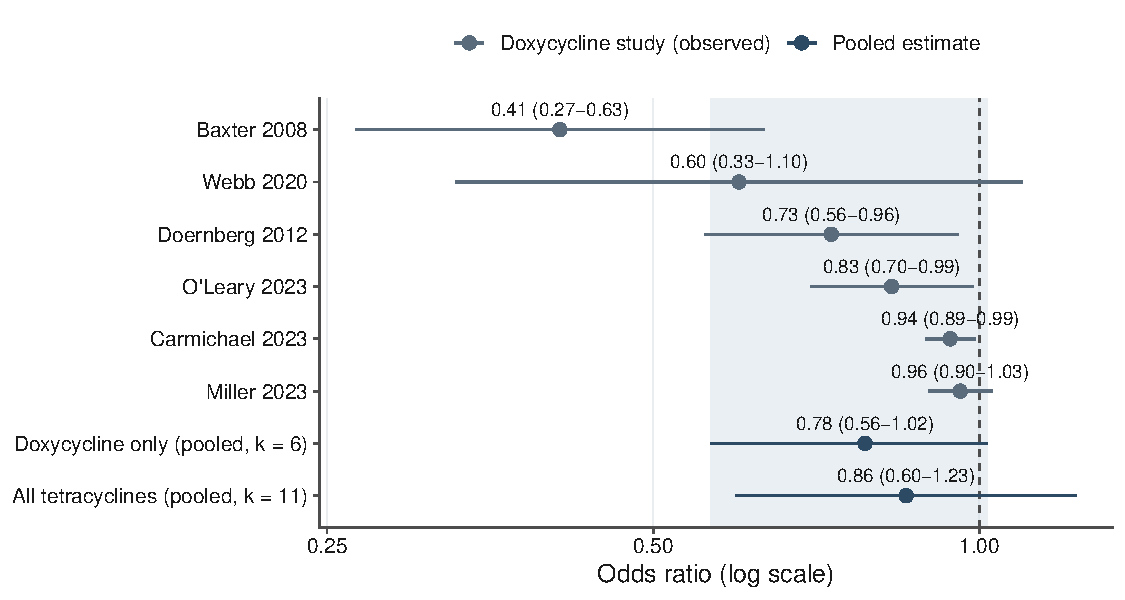
\includegraphics[keepaspectratio]{report_files/figure-pdf/fig-doxy-1.pdf}}

}

\caption{\label{fig-doxy}}

\end{figure}%

\textbf{Figure 5.} Forest plot of the doxycycline-only sensitivity
analysis. Gray points are the six doxycycline-exposure studies (observed
ORs, 95\% CIs); navy points are the pooled Bayesian estimates for the
doxycycline-only subset (k = 6) and the full primary set (k = 11). The
shaded band is the doxycycline-only 95\% credible interval; the dashed
line marks OR = 1.

\textbf{Figura 5.} Forest plot dell'analisi di sensibilità sulla sola
doxiciclina. I punti grigi sono i sei studi con esposizione a
doxiciclina (OR osservati, IC 95\%); i punti navy sono le stime
bayesiane aggregate per il sottoinsieme doxiciclina (k = 6) e per il set
primario completo (k = 11). La banda ombreggiata è l'intervallo di
credibilità al 95\% della sola doxiciclina; la linea tratteggiata indica
OR = 1.

\subsection{\texorpdfstring{{Additional sensitivity analyses}{Analisi di
sensibilità
aggiuntive}}{Additional sensitivity analysesAnalisi di sensibilità aggiuntive}}\label{additional-sensitivity-analysesanalisi-di-sensibilituxe0-aggiuntive}

\textbf{Adjusted-only secondary comparison.} Restricting the
no-antibiotic comparison to the three studies with
multivariable-adjusted estimates (Delaney 2007, Dial 2008, Brown 2016)
gives OR 1.10 (0.62--1.88) (k = 3), P(OR\textless1) = 0.34 ---
consistent with the full secondary set, with a wider interval reflecting
the smaller evidence base.

\textbf{Excluding ratio-metric conversions.} The curated estimates of
Doernberg 2012 (adjusted HR), Dial 2008 (adjusted RR) and Brown 2016
(adjusted IRR) enter the analysis as ORs under a rare-outcome
approximation. Excluding them leaves the primary estimate essentially
unchanged (k = 10; OR 0.87 (0.59--1.29), P(OR\textless1) = 0.77) and the
secondary estimate likewise (k = 7; OR 1.01 (0.67--1.60),
P(OR\textless1) = 0.49). Conclusions are robust to this approximation.

\textbf{Confronto secondario con sole stime aggiustate.} Limitando il
confronto contro nessun antibiotico ai tre studi con stime aggiustate
multivariabili (Delaney 2007, Dial 2008, Brown 2016) si ottiene OR 1.10
(0.62--1.88) (k = 3), P(OR\textless1) = 0.34 --- coerente con l'intero
set secondario, con un intervallo più ampio che riflette la base di
evidenze ridotta.

\textbf{Esclusione delle conversioni da misure di tasso/rischio.} Le
stime curate di Doernberg 2012 (HR aggiustato), Dial 2008 (RR
aggiustato) e Brown 2016 (IRR aggiustato) entrano nell'analisi come OR
tramite un'approssimazione per esiti rari. Escludendole, la stima
primaria resta sostanzialmente invariata (k = 10; OR 0.87 (0.59--1.29),
P(OR\textless1) = 0.77), così come quella secondaria (k = 7; OR 1.01
(0.67--1.60), P(OR\textless1) = 0.49). Le conclusioni sono robuste
rispetto a questa approssimazione.

\subsection{\texorpdfstring{{Quantitative bias analysis: unmeasured
confounding (E-values)}{Analisi quantitativa del bias: confondimento non
misurato
(E-value)}}{Quantitative bias analysis: unmeasured confounding (E-values)Analisi quantitativa del bias: confondimento non misurato (E-value)}}\label{quantitative-bias-analysis-unmeasured-confounding-e-valuesanalisi-quantitativa-del-bias-confondimento-non-misurato-e-value}

As a quantitative bias analysis for unmeasured confounding we report
\textbf{E-values} (\citeproc{ref-VanderWeele2017EValue}{VanderWeele and
Ding 2017}) for the pooled estimates: the minimum strength of
association (on the odds-ratio scale) that an unmeasured confounder
would need to have with \emph{both} tetracycline exposure and CDI, above
and beyond the covariates already adjusted for, to fully explain away
the observed association. For the \textbf{primary comparison} (OR 0.86)
the E-value is 1.61 for the point estimate and 1.00 for the
credible-interval bound nearest the null; for the \textbf{secondary
comparison} (OR 1.06) the corresponding values are 1.30 and 1.00. Given
the modest size of the pooled effect, only moderately strong unmeasured
confounding would suffice to bring the point estimate to the null, and
still weaker confounding could shift the interval across 1 ---
consistent with the GRADE rating, which starts observational evidence at
low certainty. The E-value addresses only unmeasured confounding; it
does not capture residual confounding from imperfectly measured
covariates, selection bias, or exposure/outcome misclassification.

Come analisi quantitativa del bias da confondimento non misurato
riportiamo gli \textbf{E-value}
(\citeproc{ref-VanderWeele2017EValue}{VanderWeele and Ding 2017}) per le
stime aggregate: la forza minima di associazione (sulla scala dell'odds
ratio) che un confondente non misurato dovrebbe avere con \emph{sia}
l'esposizione alle tetracicline \emph{sia} l'ICD, al di là delle
covariate già considerate, per spiegare completamente l'associazione
osservata. Per il \textbf{confronto primario} (OR 0.86) l'E-value è 1.61
per la stima puntuale e 1.00 per l'estremo dell'intervallo di
credibilità più vicino al valore nullo; per il \textbf{confronto
secondario} (OR 1.06) i valori corrispondenti sono 1.30 e 1.00. Data
l'entità modesta dell'effetto aggregato, un confondimento non misurato
di forza solo moderata sarebbe sufficiente a portare la stima puntuale
al valore nullo, e un confondimento ancora più debole potrebbe far
attraversare 1 all'intervallo --- coerente con la valutazione GRADE, che
parte da una certezza bassa per le evidenze osservazionali. L'E-value
riguarda solo il confondimento non misurato; non cattura il
confondimento residuo da covariate misurate in modo imperfetto, il bias
di selezione o la misclassificazione di esposizione ed esito.

\begin{longtable}[]{@{}
  >{\raggedright\arraybackslash}p{(\linewidth - 6\tabcolsep) * \real{0.2466}}
  >{\raggedright\arraybackslash}p{(\linewidth - 6\tabcolsep) * \real{0.2329}}
  >{\raggedleft\arraybackslash}p{(\linewidth - 6\tabcolsep) * \real{0.2603}}
  >{\raggedleft\arraybackslash}p{(\linewidth - 6\tabcolsep) * \real{0.2603}}@{}}
\caption{}\label{tbl-evalues}\tabularnewline
\toprule\noalign{}
\begin{minipage}[b]{\linewidth}\raggedright
Study
\end{minipage} & \begin{minipage}[b]{\linewidth}\raggedright
OR (95\% CI)
\end{minipage} & \begin{minipage}[b]{\linewidth}\raggedleft
E-value (estimate)
\end{minipage} & \begin{minipage}[b]{\linewidth}\raggedleft
E-value (CI bound)
\end{minipage} \\
\midrule\noalign{}
\endfirsthead
\toprule\noalign{}
\begin{minipage}[b]{\linewidth}\raggedright
Study
\end{minipage} & \begin{minipage}[b]{\linewidth}\raggedright
OR (95\% CI)
\end{minipage} & \begin{minipage}[b]{\linewidth}\raggedleft
E-value (estimate)
\end{minipage} & \begin{minipage}[b]{\linewidth}\raggedleft
E-value (CI bound)
\end{minipage} \\
\midrule\noalign{}
\endhead
\bottomrule\noalign{}
\endlastfoot
(\citeproc{ref-Watson2018}{Watson et al. 2018}) & 0.39 (0.31--0.51) &
4.53 & 3.36 \\
(\citeproc{ref-Baxter2008}{Baxter et al. 2008}) & 0.41 (0.27--0.63) &
4.31 & 2.54 \\
(\citeproc{ref-Webb2020}{Webb et al. 2020}) & 0.60 (0.33--1.10) & 2.72 &
1.00 \\
(\citeproc{ref-Doernberg2012}{Doernberg et al. 2012}) & 0.73
(0.56--0.96) & 2.08 & 1.27 \\
(\citeproc{ref-OLeary2023}{O'Leary et al. 2023}) & 0.83 (0.70--0.99) &
1.70 & 1.13 \\
(\citeproc{ref-Boven2026}{Boven et al. 2026}) & 0.93 (0.80--1.09) & 1.36
& 1.00 \\
(\citeproc{ref-Carmichael2023}{Carmichael et al. 2023}) & 0.94
(0.89--0.99) & 1.32 & 1.10 \\
(\citeproc{ref-Kuntz2011}{Kuntz et al. 2011}) & 0.94 (0.43--2.05) & 1.32
& 1.00 \\
(\citeproc{ref-Miller2023}{Miller et al. 2023}) & 0.96 (0.90--1.03) &
1.25 & 1.00 \\
(\citeproc{ref-Adams2017}{Adams et al. 2017}) & 1.26 (0.46--3.45) & 1.83
& 1.00 \\
(\citeproc{ref-Saito2025}{Saito et al. 2025}) & 2.97 (2.44--3.62) & 5.39
& 4.30 \\
\end{longtable}

\textbf{Supplementary Table S1.} Per-study E-values for the 11 studies
in the primary comparison (tetracyclines vs other antibiotics), ordered
by odds ratio. The E-value is the minimum strength of association
(odds-ratio scale, rare-outcome approximation) that an unmeasured
confounder would need with both tetracycline exposure and CDI, beyond
the covariates adjusted for in each study, to explain away that study's
estimate (``estimate'') or to move its confidence interval to include 1
(``CI bound''; equals 1 by definition for studies whose interval already
crosses 1). All 11 primary-set estimates are covariate-adjusted, so the
E-values quantify \emph{additional} unmeasured confounding beyond each
study's adjustment set.

\textbf{Tabella supplementare S1.} E-value per studio per gli 11 studi
del confronto primario (tetracicline vs altri antibiotici), ordinati per
odds ratio. L'E-value è la forza minima di associazione (scala dell'odds
ratio, approssimazione per esiti rari) che un confondente non misurato
dovrebbe avere sia con l'esposizione alle tetracicline sia con l'ICD, al
di là delle covariate considerate in ciascuno studio, per spiegare
completamente la stima dello studio (``estimate'') o per spostare il suo
intervallo di confidenza fino a includere 1 (``CI bound''; pari a 1 per
definizione per gli studi il cui intervallo attraversa già 1). Tutte le
11 stime del set primario sono aggiustate per covariate, per cui gli
E-value quantificano un confondimento non misurato \emph{aggiuntivo}
rispetto all'insieme di aggiustamento di ciascuno studio.

\subsection{\texorpdfstring{{Secondary comparison: vs no antibiotic (9
studies)}{Confronto secondario: vs nessun antibiotico (9
studi)}}{Secondary comparison: vs no antibiotic (9 studies)Confronto secondario: vs nessun antibiotico (9 studi)}}\label{secondary-comparison-vs-no-antibiotic-9-studiesconfronto-secondario-vs-nessun-antibiotico-9-studi}

Against a \emph{no-antibiotic} comparator the association is essentially
null (\textbf{OR 1.06 (0.75--1.53)}, P(OR\textless1) = 0.36). This is
expected --- almost any antibiotic raises CDI risk relative to no
antibiotic --- and it explains why pooling these studies into the
primary set attenuated the protective signal. The two comparator
questions are distinct and should not be combined.

Rispetto a un comparatore \emph{senza antibiotico} l'associazione è
sostanzialmente nulla (\textbf{OR 1.06 (0.75--1.53)}, P(OR\textless1) =
0.36). È un risultato atteso --- quasi ogni antibiotico aumenta il
rischio di ICD rispetto a nessun antibiotico --- e spiega perché
aggregare questi studi nel set primario attenuava il segnale protettivo.
Le due domande sul comparatore sono distinte e non vanno combinate.

\subsection{\texorpdfstring{{Subgroups}{Sottogruppi}}{SubgroupsSottogruppi}}\label{subgroupssottogruppi}

Within the primary set, the doxycycline-restricted subgroup and cohort
studies lean protective, whereas case-control studies do not --- a
design-related divergence that warrants cautious interpretation.

All'interno del set primario, il sottogruppo limitato alla doxiciclina e
gli studi di coorte tendono alla protezione, mentre gli studi
caso-controllo no: una divergenza legata al disegno da interpretare con
cautela.

{

\begin{longtable}[]{@{}lccc@{}}

\caption{\label{tbl-sub-en}}

\tabularnewline

\toprule\noalign{}
Analysis & Studies (k) & OR (95\% CrI) & P(OR\textless1) \\
\midrule\noalign{}
\endhead
\bottomrule\noalign{}
\endlastfoot
Doxycycline only & 6 & 0.78 (0.56--1.02) & 0.97 \\
Case-control designs & 6 & 1.05 (0.60--1.82) & 0.42 \\
Cohort designs & 5 & 0.69 (0.46--1.03) & 0.97 \\

\end{longtable}

}

{

\begin{longtable}[]{@{}lccc@{}}

\caption{\label{tbl-sub-it}}

\tabularnewline

\toprule\noalign{}
Analisi & Studi (k) & OR (ICr 95\%) & P(OR\textless1) \\
\midrule\noalign{}
\endhead
\bottomrule\noalign{}
\endlastfoot
Solo doxiciclina & 6 & 0.78 (0.56--1.02) & 0.97 \\
Disegni caso-controllo & 6 & 1.05 (0.60--1.82) & 0.42 \\
Disegni di coorte & 5 & 0.69 (0.46--1.03) & 0.97 \\

\end{longtable}

}

\subsection{\texorpdfstring{{Care-context
meta-regression}{Meta-regressione per contesto
assistenziale}}{Care-context meta-regressionMeta-regressione per contesto assistenziale}}\label{care-context-meta-regressionmeta-regressione-per-contesto-assistenziale}

A pre-specified Bayesian meta-regression (exact, \texttt{bmr}) on the
\textbf{primary antibiotic-comparator set (k = 11)} estimates a separate
pooled OR per care context (CA 3, HA 4, mixed 4). The protective
association is concentrated in \textbf{hospital-acquired (inpatient)
settings} (OR 0.56 (0.33--0.94), P(OR\textless1) = 0.98), while
community-acquired and mixed settings straddle 1. This mirrors Tariq
(2018), whose setting subgroup found protection in inpatients (OR 0.55)
but not mixed populations (OR 0.92). As a \textbf{sensitivity analysis
on the full primary set (k = 20; CA 6, HA 9, mixed 5)}, the
hospital-acquired estimate attenuates to OR 0.79 (0.54--1.17)
(P(OR\textless1) = 0.88), because that set adds no-antibiotic-comparator
studies that dilute the setting contrast. Per-group counts are small, so
this is exploratory; residual heterogeneity remains (τ = 0.47).

Una meta-regressione bayesiana pre-specificata (esatta, \texttt{bmr})
sul \textbf{set primario con comparatore antibiotico (k = 11)} stima un
OR aggregato per ciascun contesto (CA 3, HA 4, misto 4). L'associazione
protettiva si concentra nei \textbf{contesti ospedalieri (pazienti
ricoverati)} (OR 0.56 (0.33--0.94), P(OR\textless1) = 0.98), mentre i
contesti comunitari e misti attraversano 1. Ciò rispecchia Tariq (2018),
la cui analisi per contesto trovava protezione nei ricoverati (OR 0,55)
ma non nelle popolazioni miste (OR 0,92). Come \textbf{analisi di
sensibilità sul set primario completo (k = 20; CA 6, HA 9, misto 5)}, la
stima ospedaliera si attenua a OR 0.79 (0.54--1.17) (P(OR\textless1) =
0.88), perché quel set aggiunge studi con comparatore ``nessun
antibiotico'' che diluiscono il contrasto. Le numerosità per gruppo sono
piccole, quindi è esplorativo; l'eterogeneità residua permane (τ =
0.47).

\begin{figure}

\centering{

\pandocbounded{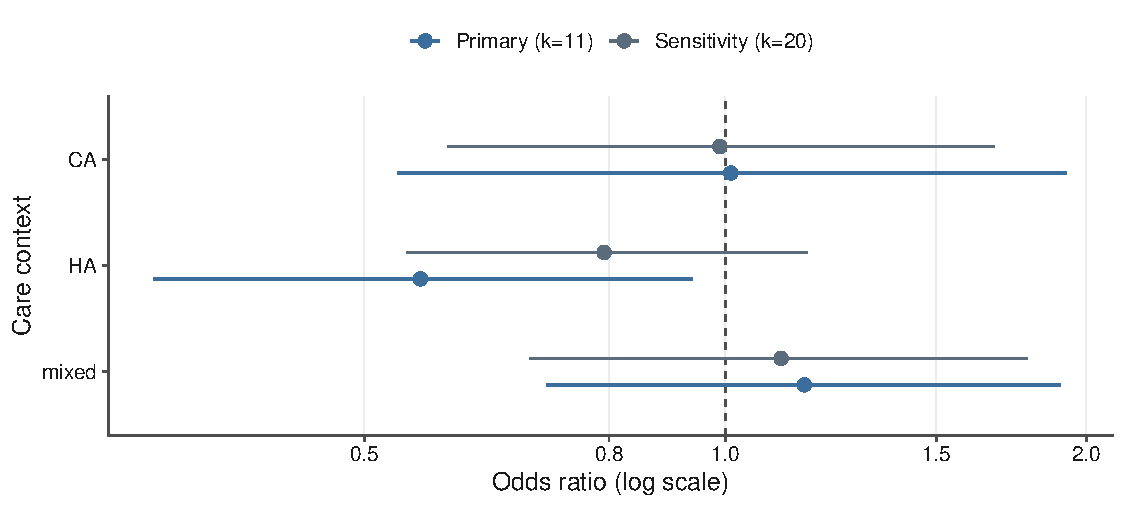
\includegraphics[keepaspectratio]{report_files/figure-pdf/fig-metareg-1.pdf}}

}

\caption{\label{fig-metareg}}

\end{figure}%

\textbf{Figure 6.} Care-context pooled ORs from the Bayesian
meta-regression: primary antibiotic-comparator set (k = 11, blue) with
full-set sensitivity (k = 20, gray).

\textbf{Figura 6.} OR aggregati per contesto dalla meta-regressione
bayesiana: set primario con comparatore antibiotico (k = 11, blu) e
sensibilità sul set completo (k = 20, grigio).

\subsection{\texorpdfstring{{Design \& adjustment
meta-regression}{Meta-regressione per disegno e
aggiustamento}}{Design \& adjustment meta-regressionMeta-regressione per disegno e aggiustamento}}\label{design-adjustment-meta-regressionmeta-regressione-per-disegno-e-aggiustamento}

Two further pre-specified Bayesian meta-regressions (exact,
\texttt{bmr}) complete the covariate set named in the protocol (§19:
context, design, adjustment). \textbf{Study design} is modelled on the
primary antibiotic-comparator set (k = 11), collapsing designs to
case-control (k = 6) versus cohort (k = 5). Cohort studies lean
protective (OR 0.69 (0.42--1.14), P(OR\textless1) = 0.93), whereas
case-control studies straddle 1 (OR 1.05 (0.65--1.70), P(OR\textless1) =
0.41) --- the same design-related divergence flagged in the subgroup
table. \textbf{Adjustment status} cannot be regressed within the primary
set because all 11 estimates are covariate-adjusted; it is therefore
assessed on the full primary set (k = 20; 14 adjusted, 6 unadjusted).
Adjusted estimates are modestly protective (OR 0.89 (0.66--1.20)) while
unadjusted estimates are null-to-slightly-adverse (OR 1.09
(0.62--1.92)), with heavily overlapping intervals that both cross 1 ---
so there is no sign that unadjusted studies inflate the protective
signal (if anything, the reverse). Per-group counts are small and
intervals wide, so both analyses are exploratory; residual heterogeneity
persists (design τ = 0.52; adjustment τ = 0.50).

Due ulteriori meta-regressioni bayesiane pre-specificate (esatte,
\texttt{bmr}) completano l'insieme di covariate indicato nel protocollo
(§19: contesto, disegno, aggiustamento). Il \textbf{disegno dello
studio} è modellato sul set primario con comparatore antibiotico (k =
11), raggruppando i disegni in caso-controllo (k = 6) vs coorte (k = 5).
Gli studi di coorte tendono alla protezione (OR 0.69 (0.42--1.14),
P(OR\textless1) = 0.93), mentre i caso-controllo attraversano 1 (OR 1.05
(0.65--1.70), P(OR\textless1) = 0.41) --- la stessa divergenza legata al
disegno evidenziata nella tabella dei sottogruppi. Lo \textbf{stato di
aggiustamento} non può essere regredito nel set primario perché tutte le
11 stime sono aggiustate; viene quindi valutato sul set primario
completo (k = 20; 14 aggiustate, 6 non aggiustate). Le stime aggiustate
sono modestamente protettive (OR 0.89 (0.66--1.20)) mentre quelle non
aggiustate sono nulle-o-lievemente-avverse (OR 1.09 (0.62--1.92)), con
intervalli ampiamente sovrapposti che attraversano entrambi 1 --- quindi
non vi è segno che gli studi non aggiustati amplifichino il segnale
protettivo (semmai il contrario). Le numerosità per gruppo sono piccole
e gli intervalli ampi, quindi entrambe le analisi sono esplorative;
l'eterogeneità residua permane (τ disegno = 0.52; τ aggiustamento =
0.50).

\begin{figure}

\centering{

\pandocbounded{
\includegraphics[keepaspectratio]{report_files/figure-pdf/fig-metareg2-1.pdf}}

}

\caption{\label{fig-metareg2}}

\end{figure}%

\textbf{Figure 7.} Pooled odds ratios from the design and adjustment
Bayesian meta-regressions (exact \texttt{bmr}, cell-means coding): study
design on the primary antibiotic-comparator set (k = 11), adjustment on
the full primary set (k = 20). Dashed line at OR = 1; all credible
intervals cross it.

\textbf{Figura 7.} OR aggregati dalle meta-regressioni bayesiane per
disegno e aggiustamento (\texttt{bmr} esatto, codifica cell-means):
disegno sul set primario con comparatore antibiotico (k = 11),
aggiustamento sul set primario completo (k = 20). Linea tratteggiata a
OR = 1; tutti gli intervalli di credibilità la attraversano.

{

\begin{longtable}[]{@{}
  >{\raggedright\arraybackslash}p{(\linewidth - 8\tabcolsep) * \real{0.2933}}
  >{\raggedright\arraybackslash}p{(\linewidth - 8\tabcolsep) * \real{0.1733}}
  >{\centering\arraybackslash}p{(\linewidth - 8\tabcolsep) * \real{0.1733}}
  >{\centering\arraybackslash}p{(\linewidth - 8\tabcolsep) * \real{0.2400}}
  >{\centering\arraybackslash}p{(\linewidth - 8\tabcolsep) * \real{0.1200}}@{}}

\caption{\label{tbl-mr2-en}}

\tabularnewline

\toprule\noalign{}
\begin{minipage}[b]{\linewidth}\raggedright
Covariate
\end{minipage} & \begin{minipage}[b]{\linewidth}\raggedright
Group
\end{minipage} & \begin{minipage}[b]{\linewidth}\centering
Studies (k)
\end{minipage} & \begin{minipage}[b]{\linewidth}\centering
OR (95\% CrI)
\end{minipage} & \begin{minipage}[b]{\linewidth}\centering
P(OR\textless1)
\end{minipage} \\
\midrule\noalign{}
\endhead
\bottomrule\noalign{}
\endlastfoot
Study design (k = 11) & Case-control & 6 & 1.05 (0.65--1.70) & 0.41 \\
Study design (k = 11) & Cohort & 5 & 0.69 (0.42--1.14) & 0.93 \\
Adjustment (k = 20) & Adjusted & 14 & 0.89 (0.66--1.20) & 0.79 \\
Adjustment (k = 20) & Unadjusted & 6 & 1.09 (0.62--1.92) & 0.39 \\

\end{longtable}

}

{

\begin{longtable}[]{@{}
  >{\raggedright\arraybackslash}p{(\linewidth - 8\tabcolsep) * \real{0.3108}}
  >{\raggedright\arraybackslash}p{(\linewidth - 8\tabcolsep) * \real{0.1757}}
  >{\centering\arraybackslash}p{(\linewidth - 8\tabcolsep) * \real{0.1486}}
  >{\centering\arraybackslash}p{(\linewidth - 8\tabcolsep) * \real{0.2432}}
  >{\centering\arraybackslash}p{(\linewidth - 8\tabcolsep) * \real{0.1216}}@{}}

\caption{\label{tbl-mr2-it}}

\tabularnewline

\toprule\noalign{}
\begin{minipage}[b]{\linewidth}\raggedright
Covariata
\end{minipage} & \begin{minipage}[b]{\linewidth}\raggedright
Gruppo
\end{minipage} & \begin{minipage}[b]{\linewidth}\centering
Studi (k)
\end{minipage} & \begin{minipage}[b]{\linewidth}\centering
OR (ICr 95\%)
\end{minipage} & \begin{minipage}[b]{\linewidth}\centering
P(OR\textless1)
\end{minipage} \\
\midrule\noalign{}
\endhead
\bottomrule\noalign{}
\endlastfoot
Disegno (k = 11) & Case-control & 6 & 1.05 (0.65--1.70) & 0.41 \\
Disegno (k = 11) & Cohort & 5 & 0.69 (0.42--1.14) & 0.93 \\
Aggiustamento (k = 20) & Adjusted & 14 & 0.89 (0.66--1.20) & 0.79 \\
Aggiustamento (k = 20) & Unadjusted & 6 & 1.09 (0.62--1.92) & 0.39 \\

\end{longtable}

}

\textbf{Design and adjustment meta-regression.} Pooled ORs per group
(exact Bayesian \texttt{bmr}, cell-means coding). Design is modelled on
the primary antibiotic-comparator set (k = 11); adjustment on the full
primary set (k = 20), because all 11 primary-comparator estimates are
adjusted. Both are exploratory given small per-group counts.

\textbf{Meta-regressione per disegno e aggiustamento.} OR aggregati per
gruppo (\texttt{bmr} bayesiano esatto, codifica cell-means). Il disegno
è modellato sul set primario con comparatore antibiotico (k = 11);
l'aggiustamento sul set primario completo (k = 20), poiché tutte le 11
stime con comparatore antibiotico sono aggiustate. Entrambe sono
esplorative viste le piccole numerosità per gruppo.

\subsection{\texorpdfstring{{Comparison with Tariq (2018)}{Confronto con
Tariq
(2018)}}{Comparison with Tariq (2018)Confronto con Tariq (2018)}}\label{comparison-with-tariq-2018confronto-con-tariq-2018}

\textbf{Can our Bayesian approach reproduce Tariq?} Yes. Applied to
Tariq's exact six studies, a DerSimonian-Laird model reproduces their
result exactly (0.62 (0.47--0.81), I² = 53\%), and our Bayesian model
gives a near-identical point estimate (0.63 (0.45--0.94),
P(OR\textless1) = 0.98). The Bayesian credible interval is wider than
Tariq's confidence interval because it propagates the uncertainty in τ
that is unavoidable with only six studies --- the divergence is one of
honest uncertainty, not of the point estimate.

\textbf{Why does the updated review not find clear protection?} Chiefly
the \textbf{additional studies}. Adding the eight newer
antibiotic-comparator studies to Tariq's six moves the pooled OR from
\textasciitilde0.63 to 0.82 (0.60--1.13) (P(OR\textless1) = 0.89) and
roughly doubles heterogeneity --- and this bridge lands essentially on
our primary estimate. The new evidence is dominated by very large
administrative cohorts (e.g.~Carmichael, Miller, Watson, Webb, Boven)
whose estimates sit close to the null and carry substantial weight.
Secondary contributors to the difference are (i) the \textbf{method}
(Bayesian vs DL), which mainly widens intervals rather than shifting the
centre; and (ii) \textbf{comparator and estimate decisions} --- our
protocol separates ``vs other antibiotics'' from ``vs no antibiotic'',
so three of Tariq's six studies (Delaney, Dial, Tartof) move to the
secondary set, and Tartof's estimate differs (Tariq's adjusted OR 0.50
vs our unadjusted 0.84).

\textbf{Il nostro approccio bayesiano riproduce Tariq?} Sì. Applicato ai
sei studi esatti di Tariq, un modello DerSimonian-Laird ne riproduce
esattamente il risultato (0.62 (0.47--0.81), I² = 53\%), e il nostro
modello bayesiano fornisce una stima puntuale quasi identica (0.63
(0.45--0.94), P(OR\textless1) = 0.98). L'intervallo di credibilità
bayesiano è più ampio dell'intervallo di confidenza di Tariq perché
propaga l'incertezza su τ, inevitabile con soli sei studi: la differenza
riguarda l'incertezza, non la stima puntuale.

\textbf{Perché la revisione aggiornata non trova una protezione netta?}
Soprattutto per gli \textbf{studi aggiuntivi}. Aggiungendo gli otto
nuovi studi con comparatore antibiotico ai sei di Tariq, l'OR aggregato
passa da \textasciitilde0,63 a 0.82 (0.60--1.13) (P(OR\textless1) =
0.89) e l'eterogeneità circa raddoppia --- e questo ``ponte'' coincide
sostanzialmente con la nostra stima primaria. Le nuove evidenze sono
dominate da coorti amministrative molto grandi (es. Carmichael, Miller,
Watson, Webb, Boven), con stime vicine al valore nullo e peso
sostanziale. Contribuiscono in via secondaria (i) il \textbf{metodo}
(bayesiano vs DL), che allarga gli intervalli più che spostare il
centro; e (ii) le \textbf{decisioni su comparatore e stime} --- il
protocollo separa ``vs altri antibiotici'' da ``vs nessun antibiotico'',
per cui tre dei sei studi di Tariq (Delaney, Dial, Tartof) passano al
set secondario, e la stima di Tartof differisce (OR aggiustato 0,50 di
Tariq vs 0,84 non aggiustato nostro).

\begin{figure}

\centering{

\pandocbounded{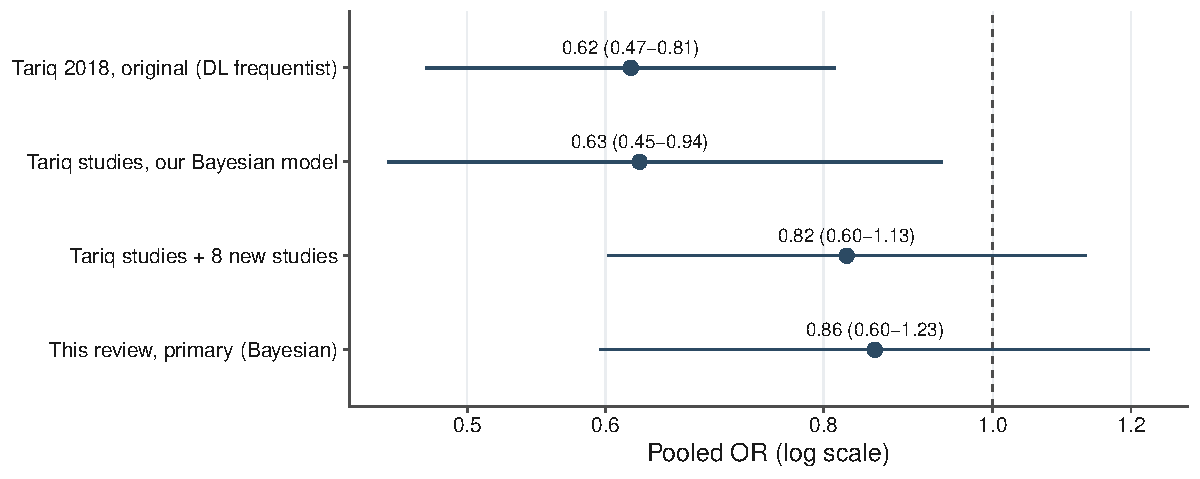
\includegraphics[keepaspectratio]{report_files/figure-pdf/fig-tariq-1.pdf}}

}

\caption{\label{fig-tariq}}

\end{figure}%

\textbf{Figure 8.} From Tariq to the updated review: recapitulation and
stepwise decomposition of the difference.

\textbf{Figura 8.} Da Tariq alla revisione aggiornata: recupero e
decomposizione passo-passo della differenza.

\subsection{\texorpdfstring{{Risk-of-bias summary}{Sintesi del rischio
di
bias}}{Risk-of-bias summarySintesi del rischio di bias}}\label{risk-of-bias-summarysintesi-del-rischio-di-bias}

Figure 9 summarises the study-level Newcastle-Ottawa judgements as a
traffic-light plot, mapping each study's per-domain star counts to Low /
Some concerns / High. All 20 studies are \textbf{Low} overall except
Predrag 2016 (some concerns); the scattered amber cells sit in the
Comparability domain (matching or adjustment credited with a single
star) and in the Outcome/Exposure domain (follow-up completeness /
non-response), while the Selection domain is green throughout except for
Predrag 2016.

La Figura 9 riassume le valutazioni Newcastle-Ottawa per studio come
traffic-light plot, mappando i conteggi di stelle per dominio in Basso /
Alcune perplessità / Alto. Tutti i 20 studi sono complessivamente a
rischio \textbf{basso} tranne Predrag 2016 (alcune perplessità); le
celle ambra si distribuiscono tra il dominio di Comparabilità
(appaiamento o aggiustamento accreditato con una sola stella) e il
dominio Esito/Esposizione (completezza del follow-up / non-risposta),
mentre il dominio di Selezione è interamente verde fatta eccezione per
Predrag 2016.

\begin{figure}

\centering{

\pandocbounded{
\includegraphics[keepaspectratio]{report_files/figure-pdf/fig-rob-1.pdf}}

}

\caption{\label{fig-rob}}

\end{figure}%

\textbf{Figure 9.} Risk-of-bias traffic-light plot (Newcastle-Ottawa
Scale). Per-domain judgements are derived from item stars --- Selection
(max 4), Comparability (max 2), Outcome/Exposure (max 3) --- and Overall
is the study-level NOS rating. Domain rules: Selection low with at least
3 of 4 stars, some concerns with 2; Comparability low with 2 stars, some
concerns with 1; Outcome/Exposure low with 3 stars, some concerns with
2; Overall 7--9 stars = low, 5--6 = some concerns, 4 or fewer = high.
Green \textbf{+} = low, amber \textbf{−} = some concerns, red \textbf{×}
= high. Provisional, single-reviewer assessment.

\textbf{Figura 9.} Traffic-light plot del rischio di bias (scala
Newcastle-Ottawa). I giudizi per dominio derivano dalle stelle per item
--- Selezione (max 4), Comparabilità (max 2), Esito/Esposizione (max 3)
--- e il giudizio complessivo è la valutazione NOS per studio. Regole
per dominio: Selezione bassa con almeno 3 stelle su 4, alcune
perplessità con 2; Comparabilità bassa con 2 stelle, alcune perplessità
con 1; Esito/Esposizione bassa con 3 stelle, alcune perplessità con 2;
Complessivo 7--9 stelle = basso, 5--6 = alcune perplessità, 4 o meno =
alto. Verde \textbf{+} = basso, ambra \textbf{−} = alcune perplessità,
rosso \textbf{×} = alto. Valutazione provvisoria, singolo revisore.

\subsection{\texorpdfstring{{Certainty of evidence (GRADE)}{Certezza
delle evidenze
(GRADE)}}{Certainty of evidence (GRADE)Certezza delle evidenze (GRADE)}}\label{certainty-of-evidence-gradecertezza-delle-evidenze-grade}

Certainty was rated following the GRADE approach
(\citeproc{ref-Guyatt2008GRADE}{Guyatt et al. 2008}). Because all
evidence is observational, both comparisons start at \emph{low}
certainty; each was rated down for serious inconsistency and serious
imprecision, yielding \textbf{very low} certainty for both questions.
The quantitative bias analysis for unmeasured confounding reinforces
this rating: the E-value for the primary pooled estimate is 1.61 (1.00
for the interval bound nearest the null), so an unmeasured confounder
only moderately associated with both tetracycline exposure and CDI ---
beyond the covariates already adjusted for --- would suffice to explain
away the association; the corresponding thresholds for the secondary
comparison are 1.30 and 1.00. The effect is therefore not large enough
to consider rating up, and residual confounding remains a live
explanation.

{\def\LTcaptype{none} % do not increment counter
\begin{longtable}[]{@{}
  >{\raggedright\arraybackslash}p{(\linewidth - 18\tabcolsep) * \real{0.1000}}
  >{\raggedright\arraybackslash}p{(\linewidth - 18\tabcolsep) * \real{0.1000}}
  >{\raggedright\arraybackslash}p{(\linewidth - 18\tabcolsep) * \real{0.1000}}
  >{\raggedright\arraybackslash}p{(\linewidth - 18\tabcolsep) * \real{0.1000}}
  >{\raggedright\arraybackslash}p{(\linewidth - 18\tabcolsep) * \real{0.1000}}
  >{\raggedright\arraybackslash}p{(\linewidth - 18\tabcolsep) * \real{0.1000}}
  >{\raggedright\arraybackslash}p{(\linewidth - 18\tabcolsep) * \real{0.1000}}
  >{\raggedright\arraybackslash}p{(\linewidth - 18\tabcolsep) * \real{0.1000}}
  >{\raggedright\arraybackslash}p{(\linewidth - 18\tabcolsep) * \real{0.1000}}
  >{\raggedright\arraybackslash}p{(\linewidth - 18\tabcolsep) * \real{0.1000}}@{}}
\toprule\noalign{}
\begin{minipage}[b]{\linewidth}\raggedright
Outcome: incident CDI
\end{minipage} & \begin{minipage}[b]{\linewidth}\raggedright
k
\end{minipage} & \begin{minipage}[b]{\linewidth}\raggedright
Pooled OR (95\% CrI)
\end{minipage} & \begin{minipage}[b]{\linewidth}\raggedright
Illustrative absolute effect*
\end{minipage} & \begin{minipage}[b]{\linewidth}\raggedright
Risk of bias
\end{minipage} & \begin{minipage}[b]{\linewidth}\raggedright
Inconsistency
\end{minipage} & \begin{minipage}[b]{\linewidth}\raggedright
Indirectness
\end{minipage} & \begin{minipage}[b]{\linewidth}\raggedright
Imprecision
\end{minipage} & \begin{minipage}[b]{\linewidth}\raggedright
Publication bias
\end{minipage} & \begin{minipage}[b]{\linewidth}\raggedright
Certainty
\end{minipage} \\
\midrule\noalign{}
\endhead
\bottomrule\noalign{}
\endlastfoot
Tetracyclines vs other antibiotics & 11 & 0.86 (0.60--1.23) & 17 vs 20
per 1,000 (12--24) & Not seriousᵃ & Seriousᵇ & Not serious & Seriousᶜ &
Undetectedᵈ & \textbf{Very low} \\
Tetracyclines vs no antibiotic & 9 & 1.06 (0.75--1.53) & 5 vs 5 per
1,000 (4--8) & Not seriousᵃ & Seriousᵇ & Seriousᵉ & Seriousᶜ &
Undetectedᵈ & \textbf{Very low} \\
\end{longtable}
}

* Illustrative only: assumes a baseline risk of 20 per 1,000
antibiotic-exposed patients (hospital context) and 5 per 1,000 unexposed
patients; absolute effects scale with the baseline risk. ᵃ All 11
primary and 8 of 9 secondary studies at low risk of bias on the
Newcastle-Ottawa Scale (provisional, single-reviewer assessment). ᵇ
Substantial heterogeneity: primary I² = 98\% (95\% CrI 96--99\%); the
predictive interval spans protection to harm. ᶜ Credible interval
includes both meaningful benefit and harm. ᵈ No funnel-plot asymmetry
(Egger's test p = 0.78), though power to detect it is limited. ᵉ The
no-antibiotic comparator answers a different question and is highly
prone to confounding by indication.

La certezza è stata valutata secondo l'approccio GRADE
(\citeproc{ref-Guyatt2008GRADE}{Guyatt et al. 2008}). Poiché tutte le
evidenze sono osservazionali, entrambi i confronti partono da una
certezza \emph{bassa}; ciascuno è stato declassato per inconsistenza e
imprecisione serie, risultando in una certezza \textbf{molto bassa} per
entrambe le domande. L'analisi quantitativa del bias da confondimento
non misurato rafforza questa valutazione: l'E-value per la stima
aggregata primaria è 1.61 (1.00 per l'estremo dell'intervallo più vicino
al valore nullo), per cui un confondente non misurato solo moderatamente
associato sia all'esposizione alle tetracicline sia all'ICD --- al di là
delle covariate già considerate --- sarebbe sufficiente a spiegare
l'associazione; le soglie corrispondenti per il confronto secondario
sono 1.30 e 1.00. L'effetto non è quindi abbastanza grande da
giustificare un aumento di certezza, e il confondimento residuo resta
una spiegazione plausibile.

{\def\LTcaptype{none} % do not increment counter
\begin{longtable}[]{@{}
  >{\raggedright\arraybackslash}p{(\linewidth - 18\tabcolsep) * \real{0.1000}}
  >{\raggedright\arraybackslash}p{(\linewidth - 18\tabcolsep) * \real{0.1000}}
  >{\raggedright\arraybackslash}p{(\linewidth - 18\tabcolsep) * \real{0.1000}}
  >{\raggedright\arraybackslash}p{(\linewidth - 18\tabcolsep) * \real{0.1000}}
  >{\raggedright\arraybackslash}p{(\linewidth - 18\tabcolsep) * \real{0.1000}}
  >{\raggedright\arraybackslash}p{(\linewidth - 18\tabcolsep) * \real{0.1000}}
  >{\raggedright\arraybackslash}p{(\linewidth - 18\tabcolsep) * \real{0.1000}}
  >{\raggedright\arraybackslash}p{(\linewidth - 18\tabcolsep) * \real{0.1000}}
  >{\raggedright\arraybackslash}p{(\linewidth - 18\tabcolsep) * \real{0.1000}}
  >{\raggedright\arraybackslash}p{(\linewidth - 18\tabcolsep) * \real{0.1000}}@{}}
\toprule\noalign{}
\begin{minipage}[b]{\linewidth}\raggedright
Esito: ICD incidente
\end{minipage} & \begin{minipage}[b]{\linewidth}\raggedright
k
\end{minipage} & \begin{minipage}[b]{\linewidth}\raggedright
OR aggregato (ICr 95\%)
\end{minipage} & \begin{minipage}[b]{\linewidth}\raggedright
Effetto assoluto illustrativo*
\end{minipage} & \begin{minipage}[b]{\linewidth}\raggedright
Rischio di bias
\end{minipage} & \begin{minipage}[b]{\linewidth}\raggedright
Inconsistenza
\end{minipage} & \begin{minipage}[b]{\linewidth}\raggedright
Indirettezza
\end{minipage} & \begin{minipage}[b]{\linewidth}\raggedright
Imprecisione
\end{minipage} & \begin{minipage}[b]{\linewidth}\raggedright
Bias di pubblicazione
\end{minipage} & \begin{minipage}[b]{\linewidth}\raggedright
Certezza
\end{minipage} \\
\midrule\noalign{}
\endhead
\bottomrule\noalign{}
\endlastfoot
Tetracicline vs altri antibiotici & 11 & 0.86 (0.60--1.23) & 17 vs 20
per 1,000 (12--24) & Non serioᵃ & Serioᵇ & Non serio & Serioᶜ & Non
rilevatoᵈ & \textbf{Molto bassa} \\
Tetracicline vs nessun antibiotico & 9 & 1.06 (0.75--1.53) & 5 vs 5 per
1,000 (4--8) & Non serioᵃ & Serioᵇ & Serioᵉ & Serioᶜ & Non rilevatoᵈ &
\textbf{Molto bassa} \\
\end{longtable}
}

* Solo illustrativo: assume un rischio di base di 20 per 1.000 pazienti
esposti ad antibiotici (contesto ospedaliero) e di 5 per 1.000 non
esposti; gli effetti assoluti variano con il rischio di base. ᵃ Tutti
gli 11 studi primari e 8 dei 9 secondari a basso rischio di bias secondo
la scala Newcastle-Ottawa (valutazione provvisoria, singolo revisore). ᵇ
Eterogeneità sostanziale: I² primario = 98\% (95\% CrI 96--99\%);
l'intervallo predittivo spazia dalla protezione al danno. ᶜ L'intervallo
di credibilità include sia un beneficio sia un danno rilevanti. ᵈ
Nessuna asimmetria del funnel plot (test di Egger p = 0.78), sebbene la
potenza per rilevarla sia limitata. ᵉ Il comparatore senza antibiotico
risponde a una domanda diversa ed è fortemente soggetto a confondimento
per indicazione.

\subsection{\texorpdfstring{{Interpretation}{Interpretazione}}{InterpretationInterpretazione}}\label{interpretationinterpretazione}

Restricted to the protocol's intended comparator (another antibiotic),
the data provide \textbf{suggestive but uncertain} evidence that
tetracycline exposure lowers CDI risk. The pooled odds ratio is below 1
(OR 0.86 (0.60--1.23)) but its 95\% credible interval still includes no
effect; the posterior probability of \emph{any} reduction is 81\%,
falling to 35\% for a clinically meaningful one (OR \textless{} 0.80).
These findings distinguish a plausibly \emph{lower associated risk} from
established \emph{protective therapy}.

\textbf{What the model fit tells us.} The random-effects model describes
the studies well, but its most informative output is the between-study
spread rather than the mean. Heterogeneity is substantial (\(\tau\) =
0.55, I² = 98\% (95\% CrI 96--99\%)), so the pooled OR summarises a
\emph{distribution} of study-specific effects rather than one common
value: the predictive interval for a new study (OR 0.25--2.88) reaches
from meaningful protection to modest harm. The partial pooling visible
in Figure 1 shrinks imprecise study estimates toward that distribution,
which is why the pooled interval is wider than a fixed-effect analysis
would imply. The exact numerical posterior was reproduced by independent
Hamiltonian Monte Carlo (R-hat ≈ 1.00, effective sample sizes in the
thousands, 0 divergent transitions), so this width faithfully reflects
the evidence rather than any artefact of computation or prior choice.

\textbf{How robust is the result?} The direction of effect is stable
across the pre-specified checks: no single study drives it
(leave-one-out OR 0.75--0.93), it persists after excluding the three
RR/HR/IRR-to-OR conversions (OR 0.87 (0.59--1.29)) and after restricting
to low-risk-of-bias studies, and there is no funnel asymmetry (Egger p =
0.78). It is likewise stable across the data-dominated priors (primary,
vague, sceptical). The only assumption that renders the result
confidently protective is the literature-informed prior centred on
Tariq's OR 0.62; the formal prior-data conflict check finds only mild
tension (z = -1.50, p = 0.13), so that shift reflects the prior's
narrowness rather than incompatibility with the updated data. The
strongest internal signals --- the doxycycline-only subset (OR 0.78
(0.56--1.02)) and hospital-acquired settings --- are consistent with a
real but small effect concentrated in specific agents and contexts, yet
each interval still touches 1.

Limitandosi al comparatore previsto dal protocollo (un altro
antibiotico), i dati forniscono un'evidenza \textbf{suggestiva ma
incerta} che l'esposizione alle tetracicline riduca il rischio di ICD.
L'odds ratio aggregato è inferiore a 1 (OR 0.86 (0.60--1.23)) ma il suo
intervallo di credibilità al 95\% include ancora l'assenza di effetto;
la probabilità a posteriori di \emph{una qualsiasi} riduzione è 81\%, e
scende al 35\% per una riduzione clinicamente rilevante (OR \textless{}
0,80). Questi risultati distinguono un plausibile \emph{minor rischio
associato} da una \emph{terapia protettiva} consolidata.

\textbf{Cosa indica l'adattamento del modello.} Il modello a effetti
casuali descrive bene gli studi, ma il suo esito più informativo è la
dispersione tra studi, non la media. L'eterogeneità è sostanziale
(\(\tau\) = 0.55, I² = 98\% (95\% CrI 96--99\%)), per cui l'OR aggregato
riassume una \emph{distribuzione} di effetti specifici per studio, non
un unico valore comune: l'intervallo predittivo per un nuovo studio (OR
0.25--2.88) va da una protezione rilevante a un modesto danno. Il
partial pooling visibile nella Figura 1 attrae le stime imprecise verso
quella distribuzione, ed è per questo che l'intervallo aggregato è più
ampio di quanto suggerirebbe un'analisi a effetti fissi. La posteriori
numerica esatta è stata riprodotta da Hamiltonian Monte Carlo
indipendente (R-hat ≈ 1,00, dimensioni campionarie efficaci nell'ordine
delle migliaia, 0 transizioni divergenti): questa ampiezza riflette
fedelmente le evidenze e non un artefatto del calcolo o della scelta del
prior.

\textbf{Quanto è robusto il risultato?} La direzione dell'effetto è
stabile in tutte le verifiche pre-specificate: nessun singolo studio la
determina (leave-one-out OR 0.75--0.93), persiste escludendo le tre
conversioni RR/HR/IRR→OR (OR 0.87 (0.59--1.29)) e limitandosi agli studi
a basso rischio di bias, e non vi è asimmetria del funnel (Egger p =
0.78). È inoltre stabile tra i prior dominati dai dati (primario, vago,
scettico). L'unica assunzione che rende il risultato decisamente
protettivo è il prior informato dalla letteratura centrato sull'OR 0,62
di Tariq; la verifica formale del conflitto prior-dati rileva solo una
lieve tensione (z = -1.50, p = 0.13), quindi tale spostamento riflette
la ristrettezza del prior e non un'incompatibilità con i dati
aggiornati. I segnali interni più marcati --- il sottoinsieme della sola
doxiciclina (OR 0.78 (0.56--1.02)) e i contesti ospedalieri --- sono
coerenti con un effetto reale ma piccolo, concentrato in agenti e
contesti specifici, benché ciascun intervallo tocchi ancora 1.

\subsection{\texorpdfstring{{What this review adds}{Cosa aggiunge questa
revisione}}{What this review addsCosa aggiunge questa revisione}}\label{what-this-review-addscosa-aggiunge-questa-revisione}

To our knowledge this is the first Bayesian re-analysis of the
tetracycline--CDI question and the first update of Tariq et al.~(2018)
with the subsequent literature: 20 studies contribute a curated effect
size (11 vs other antibiotics, 9 vs no antibiotic) drawn from 35
included reports, roughly doubling the antibiotic-comparator evidence
base.

Three features distinguish it from the earlier meta-analysis. First, it
\textbf{separates the two comparator questions} that Tariq pooled ---
tetracyclines \emph{vs other antibiotics} (the protocol's PECO) and
\emph{vs no antibiotic} --- a distinction that materially changes the
reading, because the apparent protection largely tracks the second,
confounding-prone comparison. Second, it reports the \textbf{full
posterior} --- the probabilities P(OR\textless1) and P(OR\textless0.80)
and a predictive interval --- rather than a single point estimate and
confidence interval, making the residual uncertainty and heterogeneity
explicit. Third, it adds a \textbf{pre-specified robustness programme}
(prior sensitivity, a formal prior-data conflict test, leave-one-out,
small-study diagnostics, and care-context/design/adjustment
meta-regressions) and cross-validates the exact posterior with MCMC.

Substantively, the headline is a \textbf{tempering} of the earlier
literature. Tariq's OR ≈ 0.62 reproduces exactly in our hands (0.62
(0.47--0.81)), but adding the newer, larger administrative-cohort
evidence moves the pooled estimate toward the null (0.82 (0.60--1.13)
for the combined set), and the confidently protective reading now
survives only under a prior anchored on the older result. The earlier
``low risk'' conclusion therefore appears driven partly by comparator
mixing and a smaller, earlier evidence base.

A nostra conoscenza questa è la prima ri-analisi bayesiana della
questione tetracicline--ICD e il primo aggiornamento di Tariq et
al.~(2018) con la letteratura successiva: 20 studi contribuiscono con
una stima d'effetto curata (11 vs altri antibiotici, 9 vs nessun
antibiotico) tratti da 35 report inclusi, raddoppiando all'incirca la
base di evidenze con comparatore antibiotico.

Tre elementi la distinguono dalla meta-analisi precedente. Primo,
\textbf{separa le due domande sul comparatore} che Tariq aveva aggregato
--- tetracicline \emph{vs altri antibiotici} (il PECO del protocollo) e
\emph{vs nessun antibiotico} --- una distinzione che cambia
sostanzialmente la lettura, perché la protezione apparente segue in
larga parte il secondo confronto, soggetto a confondimento. Secondo,
riporta la \textbf{posteriori completa} --- le probabilità
P(OR\textless1) e P(OR\textless0,80) e un intervallo predittivo ---
anziché una singola stima puntuale con intervallo di confidenza,
rendendo esplicite l'incertezza residua e l'eterogeneità. Terzo,
aggiunge un \textbf{programma di robustezza pre-specificato}
(sensibilità ai prior, test formale di conflitto prior-dati,
leave-one-out, diagnostica dei piccoli studi e meta-regressioni per
contesto, disegno e aggiustamento) e convalida la posteriori esatta con
MCMC.

Sul piano sostanziale, il messaggio è un \textbf{ridimensionamento}
della letteratura precedente. L'OR ≈ 0,62 di Tariq si riproduce
esattamente (0.62 (0.47--0.81)), ma l'aggiunta delle evidenze più
recenti da grandi coorti amministrative sposta la stima aggregata verso
il valore nullo (0.82 (0.60--1.13) per l'insieme combinato), e la
lettura decisamente protettiva sopravvive ora solo con un prior ancorato
al risultato precedente. La precedente conclusione di ``basso rischio''
appare quindi guidata in parte dalla mescolanza dei comparatori e da una
base di evidenze più piccola e datata.

\subsection{\texorpdfstring{{Strengths and limitations}{Punti di forza e
limiti}}{Strengths and limitationsPunti di forza e limiti}}\label{strengths-and-limitationspunti-di-forza-e-limiti}

\textbf{Strengths.} The review follows a pre-registered PROSPERO
protocol and separates comparators in line with its PECO. The Bayesian
random-effects framework propagates the uncertainty in between-study
heterogeneity that frequentist point estimates tend to understate, and
expresses results as directly interpretable probabilities and a
predictive interval. The exact posterior is reproduced by independent
HMC sampling, and a broad, pre-specified sensitivity and diagnostic
suite --- prior sensitivity, prior-data conflict, leave-one-out, Egger's
test, and three meta-regressions --- is reported transparently with
fully reproducible code.

\textbf{Limitations.} All evidence is observational, so confounding by
indication cannot be excluded --- most acutely in the no-antibiotic
comparison. Screening and risk-of-bias assessment are provisional
single-reviewer judgements pending the protocol's duplicate full-text
review; the extraction covariate matrix is not yet populated; and the
curated estimates are still flagged unverified. The ``other
antibiotics'' comparator is a heterogeneous mix rather than a single
clinically matched drug, and three estimates enter as RR/HR/IRR
converted to OR under a rare-outcome approximation. Per-group counts are
small, so the subgroup and meta-regression results are exploratory.
Finally, funnel-based diagnostics have limited power at k = 11, so
publication bias cannot be excluded despite the absence of detectable
asymmetry, and neither individual-participant data nor head-to-head
comparisons against specific agents were available.

\textbf{Punti di forza.} La revisione segue un protocollo PROSPERO
pre-registrato e separa i comparatori in linea con il suo PECO. Il
modello bayesiano a effetti casuali propaga l'incertezza
sull'eterogeneità tra studi che le stime puntuali frequentiste tendono a
sottostimare, ed esprime i risultati come probabilità direttamente
interpretabili e un intervallo predittivo. La posteriori esatta è
riprodotta da campionamento HMC indipendente, e un ampio insieme
pre-specificato di analisi di sensibilità e diagnostica --- sensibilità
ai prior, conflitto prior-dati, leave-one-out, test di Egger e tre
meta-regressioni --- è riportato in modo trasparente con codice
pienamente riproducibile.

\textbf{Limiti.} Tutte le evidenze sono osservazionali, per cui il
confondimento da indicazione non può essere escluso --- in modo più
acuto nel confronto vs nessun antibiotico. Lo screening e la valutazione
del rischio di bias sono giudizi provvisori di un singolo revisore, in
attesa della doppia revisione full-text prevista dal protocollo; la
matrice delle covariate di estrazione non è ancora popolata; e le stime
curate risultano tuttora non verificate. Il comparatore ``altri
antibiotici'' è un insieme eterogeneo e non un singolo farmaco
clinicamente confrontabile, e tre stime entrano come RR/HR/IRR
convertiti in OR con un'approssimazione per esiti rari. Le numerosità
per gruppo sono piccole, quindi i risultati dei sottogruppi e delle
meta-regressioni sono esplorativi. Infine, la diagnostica basata sul
funnel ha potenza limitata con k = 11, per cui il bias di pubblicazione
non può essere escluso nonostante l'assenza di asimmetria rilevabile, e
non erano disponibili né dati individuali dei partecipanti né confronti
diretti con agenti specifici.

\subsection{\texorpdfstring{{Discussion}{Discussione}}{DiscussionDiscussione}}\label{discussiondiscussione}

\textbf{From evidence to practice.} The Interpretation above summarises
the statistical picture --- a pooled OR below 1 that remains compatible
with no effect, dominated by between-study heterogeneity, and
confidently protective only under a literature-anchored prior. What does
that support in practice?

\textbf{Is tetracycline preferable to macrolides or other agents to
reduce CDI?} Not on this evidence. First, no included study provides a
head-to-head tetracycline-versus-macrolide comparison; the comparator is
a heterogeneous mix of ``other antibiotics'', so a macrolide-specific
preference would be an extrapolation. Second, the pooled effect is
uncertain (credible interval crossing 1, substantial heterogeneity).
Third, the protective interpretation is fragile, depending on prior
belief. The defensible statement is narrower: tetracyclines ---
particularly doxycycline --- are biologically plausible lower-CDI-risk
agents and are unlikely to be worse than typical comparators, with a
\emph{possible} modest advantage. That can reasonably inform stewardship
\emph{when the spectrum required is genuinely equivalent}, but it does
not meet the bar for a formal recommendation to prefer them, and
certainly not specifically over macrolides.

\textbf{Implications for future studies.}

\begin{itemize}
\tightlist
\item
  Use active-comparator, new-user cohort designs (or target-trial
  emulation) with an explicit, clinically matched comparator ---
  e.g.~doxycycline vs a macrolide for community-acquired pneumonia ---
  rather than pooling against undifferentiated ``other antibiotics''.
\item
  Reduce confounding by indication: adjust for or match on prior CDI,
  PPI use, hospitalisation, age and comorbidity; treat case-control
  evidence cautiously given its design-related divergence.
\item
  Standardise CDI ascertainment (testing protocols, exposure and outcome
  windows) so heterogeneity reflects biology rather than measurement.
\item
  Analyse by agent (doxycycline vs minocycline vs tigecycline) to
  isolate the doxycycline signal.
\item
  Pre-register and report completely to limit publication bias, and
  consider individual-participant-data meta-analysis to resolve the
  heterogeneity the predictive interval exposes.
\item
  Where clinically and ethically appropriate, a pragmatic randomised
  trial with CDI as a pre-specified secondary outcome would provide the
  confirmatory evidence observational data cannot.
\end{itemize}

\textbf{Dalle evidenze alla pratica.} L'Interpretazione qui sopra
riassume il quadro statistico --- un OR aggregato inferiore a 1 che
resta compatibile con l'assenza di effetto, dominato dall'eterogeneità
tra studi e decisamente protettivo solo con un prior ancorato alla
letteratura. Che cosa supporta tutto ciò nella pratica?

\textbf{Le tetracicline sono preferibili ai macrolidi o ad altri agenti
per ridurre l'ICD?} Non sulla base di queste evidenze. Primo, nessuno
studio incluso fornisce un confronto diretto tetraciclina-vs-macrolide;
il comparatore è un insieme eterogeneo di ``altri antibiotici'', perciò
una preferenza specifica sui macrolidi sarebbe un'estrapolazione.
Secondo, l'effetto aggregato è incerto (intervallo di credibilità che
attraversa 1, eterogeneità sostanziale). Terzo, l'interpretazione
protettiva è fragile e dipende dalla convinzione a priori.
L'affermazione difendibile è più circoscritta: le tetracicline --- in
particolare la doxiciclina --- sono agenti biologicamente plausibili a
minor rischio di ICD ed è improbabile che siano peggiori dei comparatori
abituali, con un \emph{possibile} modesto vantaggio. Ciò può
ragionevolmente orientare la stewardship \emph{quando lo spettro
richiesto è realmente equivalente}, ma non raggiunge la soglia per una
raccomandazione formale a preferirle, e certamente non specificamente
rispetto ai macrolidi.

\textbf{Implicazioni per gli studi futuri.}

\begin{itemize}
\tightlist
\item
  Usare disegni di coorte active-comparator, new-user (o emulazione di
  target trial) con un comparatore esplicito e clinicamente
  confrontabile --- es. doxiciclina vs un macrolide nella polmonite
  acquisita in comunità --- invece di aggregare contro ``altri
  antibiotici'' indistinti.
\item
  Ridurre il confondimento da indicazione: aggiustare o appaiare per ICD
  pregressa, uso di IPP, ospedalizzazione, età e comorbidità; trattare
  con cautela le evidenze caso-controllo data la divergenza legata al
  disegno.
\item
  Standardizzare l'accertamento dell'ICD (protocolli di test, finestre
  di esposizione ed esito) affinché l'eterogeneità rifletta la biologia
  e non la misurazione.
\item
  Analizzare per agente (doxiciclina vs minociclina vs tigeciclina) per
  isolare il segnale della doxiciclina.
\item
  Pre-registrare e riportare in modo completo per limitare il
  publication bias, e valutare una meta-analisi su dati individuali dei
  partecipanti per risolvere l'eterogeneità che l'intervallo predittivo
  evidenzia.
\item
  Ove clinicamente ed eticamente appropriato, uno studio randomizzato
  pragmatico con l'ICD come esito secondario pre-specificato fornirebbe
  la conferma che i dati osservazionali non possono dare.
\end{itemize}

\begin{tcolorbox}[enhanced jigsaw, arc=.35mm, bottomrule=.15mm, bottomtitle=1mm, breakable, colback=white, colbacktitle=quarto-callout-warning-color!10!white, colframe=quarto-callout-warning-color-frame, coltitle=black, left=2mm, leftrule=.75mm, opacityback=0, opacitybacktitle=0.6, rightrule=.15mm, title=\textcolor{quarto-callout-warning-color}{\faExclamationTriangle}\hspace{0.5em}{Warning}, titlerule=0mm, toprule=.15mm, toptitle=1mm]

\textbf{Caveats.} All included studies are observational;
Newcastle-Ottawa scores are predominantly in the low-risk range, but the
assessment is provisional pending duplicate full-text review. Estimates
convert RR/HR to OR under a rare-outcome approximation. This is evidence
synthesis for research and education, not treatment guidance for
individual patients.

\textbf{Avvertenze.} Tutti gli studi inclusi sono osservazionali; i
punteggi Newcastle-Ottawa sono prevalentemente nell'intervallo di basso
rischio, ma la valutazione è provvisoria in attesa della doppia
revisione del full-text. Le stime convertono RR/HR in OR con
un'approssimazione per esiti rari. Si tratta di una sintesi delle
evidenze a scopo di ricerca ed educativo, non di una guida terapeutica
per il singolo paziente.

\end{tcolorbox}

\subsection{\texorpdfstring{{References}{Bibliografia}}{ReferencesBibliografia}}\label{referencesbibliografia}

Bibliographic entries for the studies in the synthesis are cited in
Table 1 and listed below. Author and year are taken from the extraction;
titles, journals and DOIs in \texttt{references.bib} are a scaffold to
be verified/completed by the author (Tariq 2018 and a few studies whose
DOIs came from the source files are complete).

Le voci bibliografiche degli studi nella sintesi sono citate nella
Tabella 1 ed elencate qui sotto. Autore e anno provengono
dall'estrazione; titoli, riviste e DOI in \texttt{references.bib} sono
uno scheletro da verificare/completare (Tariq 2018 e alcuni studi con
DOI dai file sorgente sono completi).

\protect\phantomsection\label{refs}
\begin{CSLReferences}{1}{1}
\bibitem[\citeproctext]{ref-Adams2017}
Adams, Daniel J., Matthew D. Eberly, Michael Rajnik, and Cade M. Nylund.
2017. {``Risk Factors for Community-Associated {Clostridium difficile}
Infection in Children.''} \emph{The Journal of Pediatrics} 186: 105--9.
\url{https://doi.org/10.1016/j.jpeds.2017.03.032}.

\bibitem[\citeproctext]{ref-Baxter2008}
Baxter, R., G. Ray, and B. Fireman. 2008. {``Case-Control Study of
Antibiotic Use and Subsequent {Clostridium difficile}--Associated
Diarrhea in Hospitalized Patients.''} \emph{Infection Control \&
Hospital Epidemiology} 29 (1): 44--50.
\url{https://doi.org/10.1086/524320}.

\bibitem[\citeproctext]{ref-Boven2026}
Boven, A., Harry Vranken, E. Vlieghe, et al. 2026. {``Commonly
Prescribed Drugs as Risk Factors for {Clostridioides difficile}
Infections: A {Swedish} Population-Based Case--Control Study.''}
\emph{Gut}, ahead of print.
\url{https://doi.org/10.1136/gutjnl-2025-337629}.

\bibitem[\citeproctext]{ref-Brown2016}
Brown, Kevin A., Makoto M. Jones, N. Daneman, et al. 2016.
{``Importation, Antibiotics, and {Clostridium difficile} Infection in
Veteran Long-Term Care: A Multilevel Case--Control Study.''}
\emph{Annals of Internal Medicine} 164 (12): 787--94.
\url{https://doi.org/10.7326/m15-1754}.

\bibitem[\citeproctext]{ref-Carmichael2023}
Carmichael, H., S. M. Asch, and E. Bendavid. 2023. {``{Clostridium
difficile} and Other Adverse Events from Overprescribed Antibiotics for
Acute Upper Respiratory Infection.''} \emph{Journal of Internal
Medicine} 293 (4): 470--80. \url{https://doi.org/10.1111/joim.13597}.

\bibitem[\citeproctext]{ref-Delaney2007}
Delaney, J. A. Chris, Sandra Dial, Alan Barkun, and Samy Suissa. 2007.
{``Antimicrobial Drugs and Community-Acquired {Clostridium
difficile}-Associated Disease, {UK}.''} \emph{Emerging Infectious
Diseases} 13 (5): 761--63. \url{https://doi.org/10.3201/eid1305.061124}.

\bibitem[\citeproctext]{ref-Dial2008}
Dial, S., A. Kezouh, A. Dascal, A. Barkun, and S. Suissa. 2008.
{``Patterns of Antibiotic Use and Risk of Hospital Admission Because of
{Clostridium difficile} Infection.''} \emph{CMAJ} 179 (8): 767--72.
\url{https://doi.org/10.1503/cmaj.071812}.

\bibitem[\citeproctext]{ref-Doernberg2012}
Doernberg, S., L. Winston, D. Deck, and H. Chambers. 2012. {``Does
Doxycycline Protect Against Development of {Clostridium difficile}
Infection?''} \emph{Clinical Infectious Diseases} 55 (5): 615--20.
\url{https://doi.org/10.1093/cid/cis457}.

\bibitem[\citeproctext]{ref-Guh2015}
Guh, A., S. Adkins, Qunna Li, et al. 2017. {``Risk Factors for
Community-Associated {Clostridium difficile} Infection in Adults: A
Case-Control Study.''} \emph{Open Forum Infectious Diseases} 4 (4):
ofx171. \url{https://doi.org/10.1093/ofid/ofx171}.

\bibitem[\citeproctext]{ref-Guyatt2008GRADE}
Guyatt, Gordon H., Andrew D. Oxman, Gunn E. Vist, et al. 2008.
{``{GRADE}: An Emerging Consensus on Rating Quality of Evidence and
Strength of Recommendations.''} \emph{BMJ} 336 (7650): 924--26.
\url{https://doi.org/10.1136/bmj.39489.470347.AD}.

\bibitem[\citeproctext]{ref-Kuntz2011}
Kuntz, Jennifer L., Elizabeth A. Chrischilles, Jane F. Pendergast,
Loreen A. Herwaldt, and Philip M. Polgreen. 2011. {``Incidence of and
Risk Factors for Community-Associated {Clostridium difficile} Infection:
A Nested Case-Control Study.''} \emph{BMC Infectious Diseases} 11 (1):
194. \url{https://doi.org/10.1186/1471-2334-11-194}.

\bibitem[\citeproctext]{ref-Miller2023}
Miller, A. C., A. Arakkal, Daniel K. Sewell, Alberto Maria Segre, Joseph
Tholany, and P. Polgreen. 2023. {``Comparison of Different Antibiotics
and the Risk for Community-Associated {Clostridioides difficile}
Infection: A Case--Control Study.''} \emph{Open Forum Infectious
Diseases} 10 (8): ofad413. \url{https://doi.org/10.1093/ofid/ofad413}.

\bibitem[\citeproctext]{ref-OLeary2023}
O'Leary, Ashley L., Arthur K. Chan, Bethany A. Wattengel, Jiachen Xu,
and K. Mergenhagen. 2023. {``Impact of Doxycycline on {Clostridioides
difficile} Infection in Patients Hospitalized with Community-Acquired
Pneumonia.''} \emph{American Journal of Infection Control} 52 (3):
280--83. \url{https://doi.org/10.1016/j.ajic.2023.09.007}.

\bibitem[\citeproctext]{ref-Saito2025}
Saito, T., Y. Sato, and S. Yamamoto. 2025. {``Antimicrobial Combinations
as Novel Indicators for {Clostridioides difficile} Infection
Development: Population-Based, Nested Case-Controlled Study in {Japan}
--- the {Shizuoka Kokuho} Database Study.''} \emph{Journal of Infection
and Chemotherapy} 31 (2): 102552.
\url{https://doi.org/10.1016/j.jiac.2024.11.002}.

\bibitem[\citeproctext]{ref-Predrag2016}
Stojanović, Predrag. 2016. {``Analysis of Risk Factors and Clinical
Manifestations Associated with {Clostridium difficile} Disease in
{Serbian} Hospitalized Patients.''} \emph{Brazilian Journal of
Microbiology} 47 (4): 902--10.
\url{https://doi.org/10.1016/j.bjm.2016.07.011}.

\bibitem[\citeproctext]{ref-Strom2017}
Ström, J., J. Tham, F. Månsson, et al. 2017. {``The Association Between
{GABA}-Modulators and {Clostridium difficile} Infection --- a Matched
Retrospective Case-Control Study.''} \emph{PLoS ONE} 12 (1): e0169386.
\url{https://doi.org/10.1371/journal.pone.0169386}.

\bibitem[\citeproctext]{ref-Tariq2018}
Tariq, Raseen, and Sahil Khanna. 2018. {``Low Risk of Primary
{Clostridium difficile} Infection with Tetracyclines: A Systematic
Review and Meta-Analysis.''} \emph{Clinical Infectious Diseases} 66 (4):
514--22. \url{https://doi.org/10.1093/cid/cix833}.

\bibitem[\citeproctext]{ref-Tartof2015}
Tartof, S., G. Rieg, R. Wei, H. Tseng, S. Jacobsen, and Kalvin C. Yu.
2015. {``A Comprehensive Assessment Across the Healthcare Continuum:
Risk of Hospital-Associated {Clostridium difficile} Infection Due to
Outpatient and Inpatient Antibiotic Exposure.''} \emph{Infection Control
\& Hospital Epidemiology} 36 (12): 1409--16.
\url{https://doi.org/10.1017/ice.2015.220}.

\bibitem[\citeproctext]{ref-Tilton2019}
Tilton, C. S., and S. W. Johnson. 2019. {``Development of a Risk
Prediction Model for Hospital-Onset {Clostridium difficile} Infection in
Patients Receiving Systemic Antibiotics.''} \emph{American Journal of
Infection Control} 47 (3): 280--84.
\url{https://doi.org/10.1016/j.ajic.2018.08.021}.

\bibitem[\citeproctext]{ref-VanderWeele2017EValue}
VanderWeele, Tyler J., and Peng Ding. 2017. {``Sensitivity Analysis in
Observational Research: Introducing the {E-Value}.''} \emph{Annals of
Internal Medicine} 167 (4): 268--74.
\url{https://doi.org/10.7326/M16-2607}.

\bibitem[\citeproctext]{ref-Watson2018}
Watson, T., J. Hickok, S. Fraker, K. Korwek, R. E. Poland, and E.
Septimus. 2018. {``Evaluating the Risk Factors for Hospital-Onset
{Clostridium difficile} Infections in a Large Healthcare System.''}
\emph{Clinical Infectious Diseases} 66 (12): 1957--59.
\url{https://doi.org/10.1093/cid/cix1112}.

\bibitem[\citeproctext]{ref-Webb2020}
Webb, B., A. Subramanian, B. Lopansri, et al. 2020. {``Antibiotic
Exposure and Risk for Hospital-Associated {Clostridioides difficile}
Infection.''} \emph{Antimicrobial Agents and Chemotherapy} 64 (4):
e02169--19. \url{https://doi.org/10.1128/aac.02169-19}.

\bibitem[\citeproctext]{ref-WellsNOS}
Wells, George A., Beverley Shea, Dianne O'Connell, et al. 2011.
\emph{The {Newcastle-Ottawa Scale} ({NOS}) for Assessing the Quality of
Nonrandomised Studies in Meta-Analyses}.
\href{http://www.ohri.ca/programs/clinical_epidemiology/oxford.asp}{Http://www.ohri.ca/programs/clinical\_epidemiology/oxford.asp}.

\bibitem[\citeproctext]{ref-Yu2021}
Yu, H., N. Flaster, A. L. Casanello, and D. Curcio. 2021. {``Assessing
Risk Factors, Mortality, and Healthcare Utilization Associated with
{Clostridioides difficile} Infection in Four {Latin American}
Countries.''} \emph{Brazilian Journal of Infectious Diseases} 25 (1):
101040. \url{https://doi.org/10.1016/j.bjid.2020.11.005}.

\end{CSLReferences}

\begin{center}\rule{0.5\linewidth}{0.5pt}\end{center}

Reproducible source: \texttt{report.qmd}. Bayesian normal-normal
hierarchical model (\texttt{bayesmeta}, exact numerical posterior),
confirmed by \texttt{brms}/Stan MCMC. Re-render with
\texttt{quarto\ render\ report.qmd}.

Sorgente riproducibile: \texttt{report.qmd}. Modello gerarchico
normale-normale bayesiano (\texttt{bayesmeta}, posteriori numerica
esatta), confermato con MCMC \texttt{brms}/Stan. Ri-generare con
\texttt{quarto\ render\ report.qmd}.




\end{document}
